\documentclass[a4paper]{article}

\usepackage{hyperref}
\usepackage{amsmath}
\usepackage{mathtools}
\usepackage[german]{babel}
\usepackage[utf8]{inputenc}
\usepackage{amsfonts}
\usepackage{graphicx}
\usepackage{siunitx}
\usepackage{tabularx}
\usepackage{wrapfig}
\usepackage{float}
\usepackage[margin=2cm]{geometry}
\usepackage{mathtools}


\DeclarePairedDelimiter\abs{\lvert}{\rvert}%
\DeclarePairedDelimiter\norm{\lVert}{\rVert}%

\makeatletter
\let\oldabs\abs
\def\abs{\@ifstar{\oldabs}{\oldabs*}}

\let\oldnorm\norm
\def\norm{\@ifstar{\oldnorm}{\oldnorm*}}
\makeatother
\newcommand*{\Value}{\frac{1}{2}x^2}

%opening
\title{Zusammenfassung Oberstufe Physik\\Drei Jahre auf 20 Seiten}
\author{Noah Peeters\\ Autor\\ \small{Schüler, Otto-Hahn-Gymnasium Geesthacht, Germany} \and Jonas Peeters\\Autor\\ \small{Schüler, Otto-Hahn-Gymnasium Geesthacht, Germany} \and Merlin Brandt\\ Lektor\\\small{Schüler, Otto-Hahn-Gymnasium Geesthacht, Germany} \and Til Blechschmidt\\Lektor\\ \small{Schüler, Otto-Hahn-Gymnasium Geesthacht, Germany} }
\date{August 2017}


\begin{document}
	
	\pagenumbering{gobble}
	
	\newgeometry{top=5cm, left=3cm, right=3cm}
	\maketitle
	
	
	\newpage
	\newgeometry{top=5cm, left=2cm, right=2cm}
	

	\begin{center}
		
		{\LARGE \textbf{Danksagung}\\[30pt]}
		An dieser Stelle möchte ich mich bei unserem Physiklehrer Herrn Stephan Wulff bedanken, der uns über die letzten zweieinhalb Jahre erfolgreich den Inhalt der folgenden Seiten beigebracht hat und und trotz der neuen Anstellung in Trittau zwei Mal die Woche nach Geesthacht kommt, um uns bis zum Ende unserer Schulzeit zu begleiten.\\
		Dabei bestand der Unterricht keinesfalls aus einschläfernden Frontalunterricht. Vielmehr wurden verschiedenste Experimente, Videos, Simulationen und die geschichtliche Entwicklung unser heutigen Physik sowie eine Vielzahl an glamourösen Überschriften in den stets strukturieren Unterricht eingebracht, bei denen es niemals an Humor fehlte.
	\end{center}
	
	\newpage
	
	\newgeometry{top=2cm, left=2cm, right=2cm}
	
	\pagenumbering{arabic}
	
	\tableofcontents
	\listoffigures
	\listoftables
	\newpage
	
	\section{Kinematik}
		\subsection{Charakteristische Größen}
			\begin{table}[H]
				\def\arraystretch{1.5}
				\begin{tabularx}{\textwidth}{|c|c|c|X|}\hline
					Größe & Einheit & Formel & Beschreibung \\\hline
					$s(t)$ & \si{\meter} & $s(t) = \frac{a}{2}\cdot t^2+v_0\cdot t+s_0$ & Die Position beschreibt, wie weit sich ein Objekt bewegt hat.\\\hline
					$v(t)$ & \si{\meter\per\second}  & $v(t) = \dot{s}(t) = a\cdot t+v_0$ & Die Geschwindigkeit beschreibt, wie schnell sich ein Objekt relativ zu einem Bezugspunkt bewegt.\\\hline
					$a(t)$ & \si{\meter\per\second\squared} & $a(t) = \dot{v}(t) = \ddot{s}(t) = a$ & Die Beschleunigung beschreibt, wie sich die Geschwindigkeit eines Objektes verändert.\\\hline
				\end{tabularx}
				\caption {Charakteristische Größen der Kinematik}
				\label{table:kinematik_grossen}
			\end{table}
		
		\subsection{Wichtige Bewegungen}
			\subsubsection{Freier Fall}
				Der freie Fall ist eine idealisierte Bewegung ohne Energieverlust oder Reibung. Auf das Objekt wirkt im freien Fall nur die Gravitationskraft einer einzigen punktförmigen Masse. Das Objekt startet bei der Höhe $h_0$ ohne eine Geschwindigkeit. Die Beschleunigung $a$ ist immer senkrecht nach unten gerichtet. Auf der Erde gilt näherungsweise $a=g\approx9.81$. Damit ergibt sich das Bewegungsgesetz
				
				\begin{equation}
					h(t) = h_0 - \frac{a}{2}\cdot t^2
				\end{equation}
			
			\subsubsection{Waagerechter Wurf}
				Der waagerechte Wurf ist wieder eine idealisierte Bewegung ohne Energieverlust oder Reibung. Auf das Objekt wirkt während des Fluges nur die Gravitationskraft einer einzigen punktförmigen Masse. Beim waagerechten Wurf startet das Objekt ebenfalls bei der Höhe $h_0$ und die Beschleunigung $a$ ist ebenfalls senkrecht nach unten gerichtet. Das Objekt startet jedoch mit einer zur Beschleunigung \textit{senkrecht} stehenden Geschwindigkeit $v_{x,0}$. Der waagerechte Wurf lässt sich als \textit{Überlagerung} zweier Bewegungen, eine in x-Richtung und eine in y-Richtung, beschreiben:
				
				\begin{equation}\label{waagerechter_wurf:h}
					h(t) = h_0 - \frac{a}{2}\cdot t^2
				\end{equation}
				
				\begin{equation}\label{waagerechter_wurf:x}
					x(t) = v_{x,0}\cdot t
				\end{equation}
				Mithilfe von Gleichung \ref{waagerechter_wurf:h} kann man nun die Zeit berechnen, die das Objekt braucht, um den Wurf zu beenden. Daf\"ur wird $h_0$ mit $0$ gleichgesetzt (unter der Annahme, dass sich auf Höhe $0$ der Boden befindet):
				
				\begin{equation}
					h(t) = 0 =  h_0 - \frac{a}{2}\cdot t^2
				\end{equation}
				\begin{equation}\label{waagerechter_wurf:t}
					t = \sqrt{\frac{2h_0}{a}}
				\end{equation}
				Setzt man nun Gleichung \ref{waagerechter_wurf:t} in Gleichung \ref{waagerechter_wurf:x} ein, erhält man die Strecke, die während des Fluges in x-Richtung zur\"uckgelegt wurde:
			
				\begin{equation}
					x(t) = v_{x,0}\cdot\sqrt{\frac{2h_0}{a}}
				\end{equation}
				
			\subsubsection{Schräger Wurf}
				Der schräge Wurf ist eine besondere Form des waagerechten Wurfs, bei dem die Geschwindigkeit nicht senkrecht zur Beschleunigung steht. Der Winkel zwischen der initialen Geschwindigkeit $v_0$ und der zur Beschleunigung senkrecht stehenden Ebene wird mit $\alpha$ bezeichnet. Nun kann man die initiale Geschwindigkeit wie folgt in ihre x und y Komponente aufgeteilt werden:
				
				\begin{equation}
					v_{x,0} = \cos(\alpha)\cdot v_0
				\end{equation}
				\begin{equation}
					v_{y,0} = \sin(\alpha)\cdot v_0
				\end{equation}
				Mit diesen beiden Geschwindigkeiten kann man wieder den Wurf als zwei \"uberlagerte Bewegungen betrachten:
				
				\begin{equation}
					h(t) = h_0 - \frac{a}{2}\cdot t^2 - v_{y,0}\cdot t = h_0 - \frac{a}{2}\cdot t^2 - \sin(\alpha)\cdot v_0\cdot t
				\end{equation}
				
				\begin{equation}
					x(t) = v_{x,0}\cdot t = \cos(\alpha)\cdot v_0\cdot t
				\end{equation}
			
	\section{Dynamik}
		\subsection{Charakteristische Größen}
	
			\begin{table}[H]
				\def\arraystretch{1.5}
				\begin{tabularx}{\textwidth}{|c|c|c|X|}\hline
					Größe & Einheit & Formel & Beschreibung \\\hline
					$\vec{p}$ & \si{\kg\meter\per\second} & $\vec{p} = m\cdot \vec{v}$ & Der Impuls.\\\hline
					$\vec{F}$ & \si{\newton}=\si{\kg\meter\per\second\squared}  & $	\vec{F} = m\cdot \vec{a}$ & Die Kraft.\\\hline
					$E$ & \si{\joule}=\si{\kg\meter\squared\per\second\squared} &\hyperref[energie_kin]{$E_{kin}$}; \hyperref[energie_pot]{$E_{Pot}$}  & Die Energie.\\\hline
				\end{tabularx}
				\caption {Charakteristische Größen der Dynamik}
				\label{table:dynamik_grossen}
			\end{table}
	
			\subsubsection{Impuls}
			
				Der Impuls lässt sich umgangssprachlich als ''Schwung'' oder ''Wucht'' beschreiben. Er ist eine vektorielle Größe und sowohl zur Masse als auch zur Geschwindigkeit eines Körpers proportional:
				
				\begin{equation}
					\vec{p} = m\cdot \vec{v}
				\end{equation}
				Da $m$ eine skalare Größe ist, sind $\vec{p}$ und $\vec{v}$ gleich ausgerichtet.\\
				Die Summe aller Impulse in einem abgeschlossenen System bleibt konstant. \\ Es gilt der Impulserhaltungssatz: $\vec{p_1} + \vec{p_2} + ... + \vec{p_n} = \vec{p} = const$.
			
			\subsubsection{Kräfte}
			
				Die Kraft ist eine vektorielle Größe und zur Masse sowie zur Beschleunigung des Körpers proportional:
				
				\begin{equation}\label{kraft:fma}
					\vec{F} = \vec{\dot{p}} = m\cdot \vec{\dot{v}} = m\cdot \vec{a}
				\end{equation}
				Da $m$ eine skalare Größe ist, sind $\vec{F}$ und $\vec{a}$ gleich ausgerichtet. Es gelten die Newton'schen Gesetze:
				
				\begin{enumerate}
					\item Wenn die Summe aller auf einen Körper wirkenden Kräfte null ist, bleibt die Geschwindigkeit konstant: $\vec{v} = const$ wenn $\vec{F} = 0$.
					\item Es gilt $\vec{F} = m\cdot \vec{a}$.
					\item Zu jeder wirkende Kraft wirkt eine ihr vom Betrag her gleich große Kraft in die entgegengesetzte Richtung: $\vec{F_1} = -\vec{F_2}$ \textit{(Actio gleich Reactio)}.
				\end{enumerate}
		
			\subsubsection{Energien in der klassischen Mechanik}
			
				Die Energie in einem abgeschlossenen System bleibt konstant. Es gilt der Energieerhaltungssatz: $\vec{E_1} + \vec{E_2} + ... + \vec{E_n} = \vec{E} = const$.\\
				Die Energie lässt sich in verschiedene Formen einteilen.
				
				\paragraph{Kinetische Energie (Bewegungsenergie)}\label{energie_kin}
					Die kinetische Energie beschreibt die Energie, die in Form von Bewegung gespeichert ist. Sie lässt sich folgendermaßen berechnen:
					
					\begin{equation}\label{energie_kin_eq}
						E_{kin} = \frac{1}{2}\cdot m\cdot v^2
					\end{equation}
					
				\paragraph{Potenzielle Energie (Lageenergie)}\label{energie_pot}
					Die potenzielle Energie beschreibt die Energie, die in der Lage oder Position einer Masse gespeichert ist. Die potenzielle Energie einer sich in einem Feld befindenden Masse mit der Beschleunigung $a$ lässt sich folgendermaßen berechnen:
					
					\begin{equation}
						E_{pot} = m\cdot a \cdot s
					\end{equation}
					Zusammen mit der Gleichung \ref{kraft:fma} erhält man:
					
					\begin{equation}\label{energie:fs}
						E_{pot} = \vec{F} \cdot s
					\end{equation}
	
		\subsection{Anwendungen}
			\subsubsection{Newtonpendel}
				Beim Newtonpendel hängen mehrere gleich schwere Kugeln mit jeweils der Masse $m$ in einer Reihe an Fäden. Hebt man nun $n_1 \in \mathbb{N}$ Kugeln seitlich hoch und lässt sie dann schwingen, sodass es einen zentralen Stoß mit den restlichen Kugeln gibt, bei der die schwingenden Kugeln die Geschwindigkeit $v$ haben, entfernen sich an der anderen Kugelreihenseite $n_2 \in \mathbb{N}$ Kugeln mit der Geschwindigkeit $u$. Um zu beweisen, dass $n_1 = n_2$ ist, muss man sowohl den Impuls- als auch den Energieerhaltungssatz anwenden, aus dem sich jedoch jeweils die Masse rauskürzen lässt:
				
				\begin{equation}\label{newtonpendel:p_short}
				\begin{aligned}
					p=n_1\cdot m \cdot v &= n_2\cdot m \cdot u\\
					n_1\cdot v &= n_2 \cdot u
				\end{aligned}
				\end{equation}
				\begin{equation}\label{newtonpendel:e_short}
				\begin{aligned}
					E=\frac{1}{2}\cdot n_1\cdot m \cdot v^2 &= \frac{1}{2}\cdot n_2\cdot m \cdot u^2\\
					n_1 \cdot v^2 &= n_2 \cdot u^2
					\end{aligned}
				\end{equation}
				Nun kann man Gleichung \ref{newtonpendel:p_short} zu $u$ umstellen, und diese anschließend in die Gleichung \ref{newtonpendel:e_short} einsetzen.
			
				\begin{equation}
					u = \frac{n_1\cdot v}{n_2}
				\end{equation}
				
				\begin{equation}
					n_1 \cdot v^2 =n_2 \cdot \left(\frac{n_1\cdot v}{n_2}\right) ^2\Leftrightarrow n_1 = n_2
				\end{equation}

	
			\subsubsection{Elastischer Stoß}
			
				Treffen zwei Körper mit den Massen $m_1$ und $m_2$ und den Geschwindigkeiten $v_1$ und $v_2$ elastisch aufeinander, kommt es zum elastischen Stoß. Wenn die Geschwindigkeiten nach dem Stoß mit $u_1$ und $u_2$ bezeichnet werden, gilt nach dem Impuls- und Energieerhaltungssatz:\\\\
				Impulserhaltung:
				\begin{equation}\label{elastischer_stoss:p}
					\begin{aligned}
					p=m_1 \cdot v_1 + m_2 \cdot v_2 &= m_1 \cdot u_1 + m_2 \cdot u_2\\
					m_1 \cdot (v_1 - u_1) &= m_2 \cdot (u_2 - v_2)
					\end{aligned}
				\end{equation}
				Energieerhaltung:
				\begin{equation}\label{elastischer_stoss:e}
					\begin{aligned}
					E=\frac{1}{2}m_1 \cdot v_1 + \frac{1}{2}m_2 \cdot v_2 &= \frac{1}{2}m_1 \cdot u_1 + \frac{1}{2}m_2 \cdot u_2\\
					m_1 \cdot (v_1^2 - u_1^2) &= m_2 \cdot (u_2^2 - v_2^2)\\
						m_1 \cdot (v_1 - u_1)(v_1 + u_1)&= m_2 \cdot (u_2 - v_2)(u_2 + v_2)
					\end{aligned}
				\end{equation}
				Nun kann man Gleichung \ref{elastischer_stoss:p} in Gleichung \ref{elastischer_stoss:e} einsetzen:
				\begin{equation}\label{elastischer_stoss:u1_u2}
					\begin{aligned}
					m_2 \cdot (u_2 - v_2)(v_1 + u_1)&= m_2 \cdot (u_2 - v_2)(u_2 + v_2)\\
					v_1 + u_1&= u_2 + v_2
					\end{aligned}
				\end{equation}
				Setzt man Gleichung \ref{elastischer_stoss:u1_u2} zu $u_2$ oder $u_1$ umgestellt in Gleichung \ref{elastischer_stoss:p} ein, erhält man Formeln für $u_1$ und $u_2$:
				
				\begin{equation}
					u_1=\frac{m_2(2v_2 - v_1) + m_1v_1}{m_1+m_2}
				\end{equation}
				\begin{equation}
					u_2=\frac{m_1(2v_1 - v_2) + m_2v_2}{m_1+m_2}
				\end{equation}
	
			\subsubsection{Unelastischer Stoß}
			
				Treffen zwei Körper mit den Massen $m_1$ und $m_2$ und den Geschwindigkeiten $v_1$ und $v_2$ unelastisch aufeinander, kommt es zum unelastischen Stoß. Das heißt, die Körper lösen sich nach dem Stoß nicht voneinander. Wenn die Geschwindigkeit des neuen Körpers nach dem Stoß mit $u$ bezeichnet wird, gilt nach dem Impulserhaltungssatz:
				
				\begin{equation}\label{unelastischer_stoss:p}
					p=m_1 \cdot v_1 + m_2 \cdot v_2 = (m_1 + m_2) \cdot u
				\end{equation}
				Für die Geschwindigkeit $u$ ergibt sich nach Gleichung \ref{unelastischer_stoss:p}:
				
				\begin{equation}
					u=\frac{m_1 \cdot v_1 + m_2 \cdot v_2}{m_1 + m_2}
				\end{equation}
			
			
	\section{Schwingungen und Wellen}			
		\subsection{Charakteristische Größen}

	
			\begin{table}[H]
				\def\arraystretch{1.5}
				 \begin{tabularx}{\textwidth}{|c|c|c|X|}\hline
					Größe & Einheit & Formel & Beschreibung \\\hline
					$T$ & \si{\second} & & Die Zeit für eine vollständige Periode.\\\hline
					$f$ & \si{\hertz}  & $\frac{1}{T}$ & Das Reziprok der Zeit für eine vollständige Periode.\\\hline
					$\lambda$ & \si{\meter} & & Die räumliche Ausdehnung einer Periode.\\\hline
					$c$ & \si{\meter\per\second} & $c=\lambda\cdot f = \frac{\lambda}{T}$ & Die Geschwindigkeit der räumlichen Ausbreitung.\\\hline
					$\hat{y}$ & \si{\meter}& & Die Amplitude der Schwingung beschreibt die maximale Auslenkung.\\\hline
					$\omega$ & \si{\hertz} & $\omega=\frac{2\pi}{T}$ & Die Winkelgeschwindigkeit des Zeigers im Zeigermodell.\\\hline
					$y(t, x)$ & \si{\meter} & $\hat{y}\cdot\sin\left(2\pi\left(\frac{t}{T}-\frac{x}{\lambda} \right)\right)$ & Die Elongation beschreibt die Auslenkung einer Welle zu einem bestimmten Zeitpunkt $t$ an einem bestimmten Ort $x$.\\\hline
					$v(t, x)$ & \si{\meter\per\second} & $\hat{y}\cdot\omega\cdot\cos\left(2\pi\left(\frac{t}{T}-\frac{x}{\lambda} \right)\right)$ & Die Geschwindigkeit beschreibt die Schwinggeschwindigkeit zu einem bestimmten Zeitpunkt $t$ an einem bestimmten Ort $x$.\\\hline
					$a(t, x)$ & \si{\meter\per\second\squared} & $-\hat{y}\cdot\omega^2\cdot\sin\left(2\pi\left(\frac{t}{T}-\frac{x}{\lambda} \right)\right)$ & Die Beschleunigung beschreibt die Schwingbeschleunigung zu einem bestimmten Zeitpunkt $t$ an einem bestimmten Ort $x$.\\\hline
				\end{tabularx}
				\caption {Charakteristische Größen für Schwingungen und Wellen}
				\label{table:wellen_grossen}
			\end{table}	
	
		\subsection{Herleitung von $y(t, x)$}
			Zum Zeitpunkt $t$ hat die Welle $\frac{t}{T}$ von einer vollen Phase also von $2\pi = 360\si{\degree}$ geschafft. Damit ist die Phase $\varphi = 2\pi\cdot\frac{t}{T} = \frac{2\pi}{T}\cdot t$. Die Elongation lässt sich mithilfe eines rechtwinkligen Dreiecks wie es in Abbildung \ref{img:welle_zeigerdarstellung} als $y=\hat{y}\cdot sin\left(\varphi\right)$ bestimmen. Damit gilt
			
			\begin{equation}\label{einfache_wellengleichung}
				y=\hat{y}\cdot sin\left(\frac{2\pi}{T}\cdot t\right)
			\end{equation}
			
			
			\begin{figure}[ht]
				\centering
				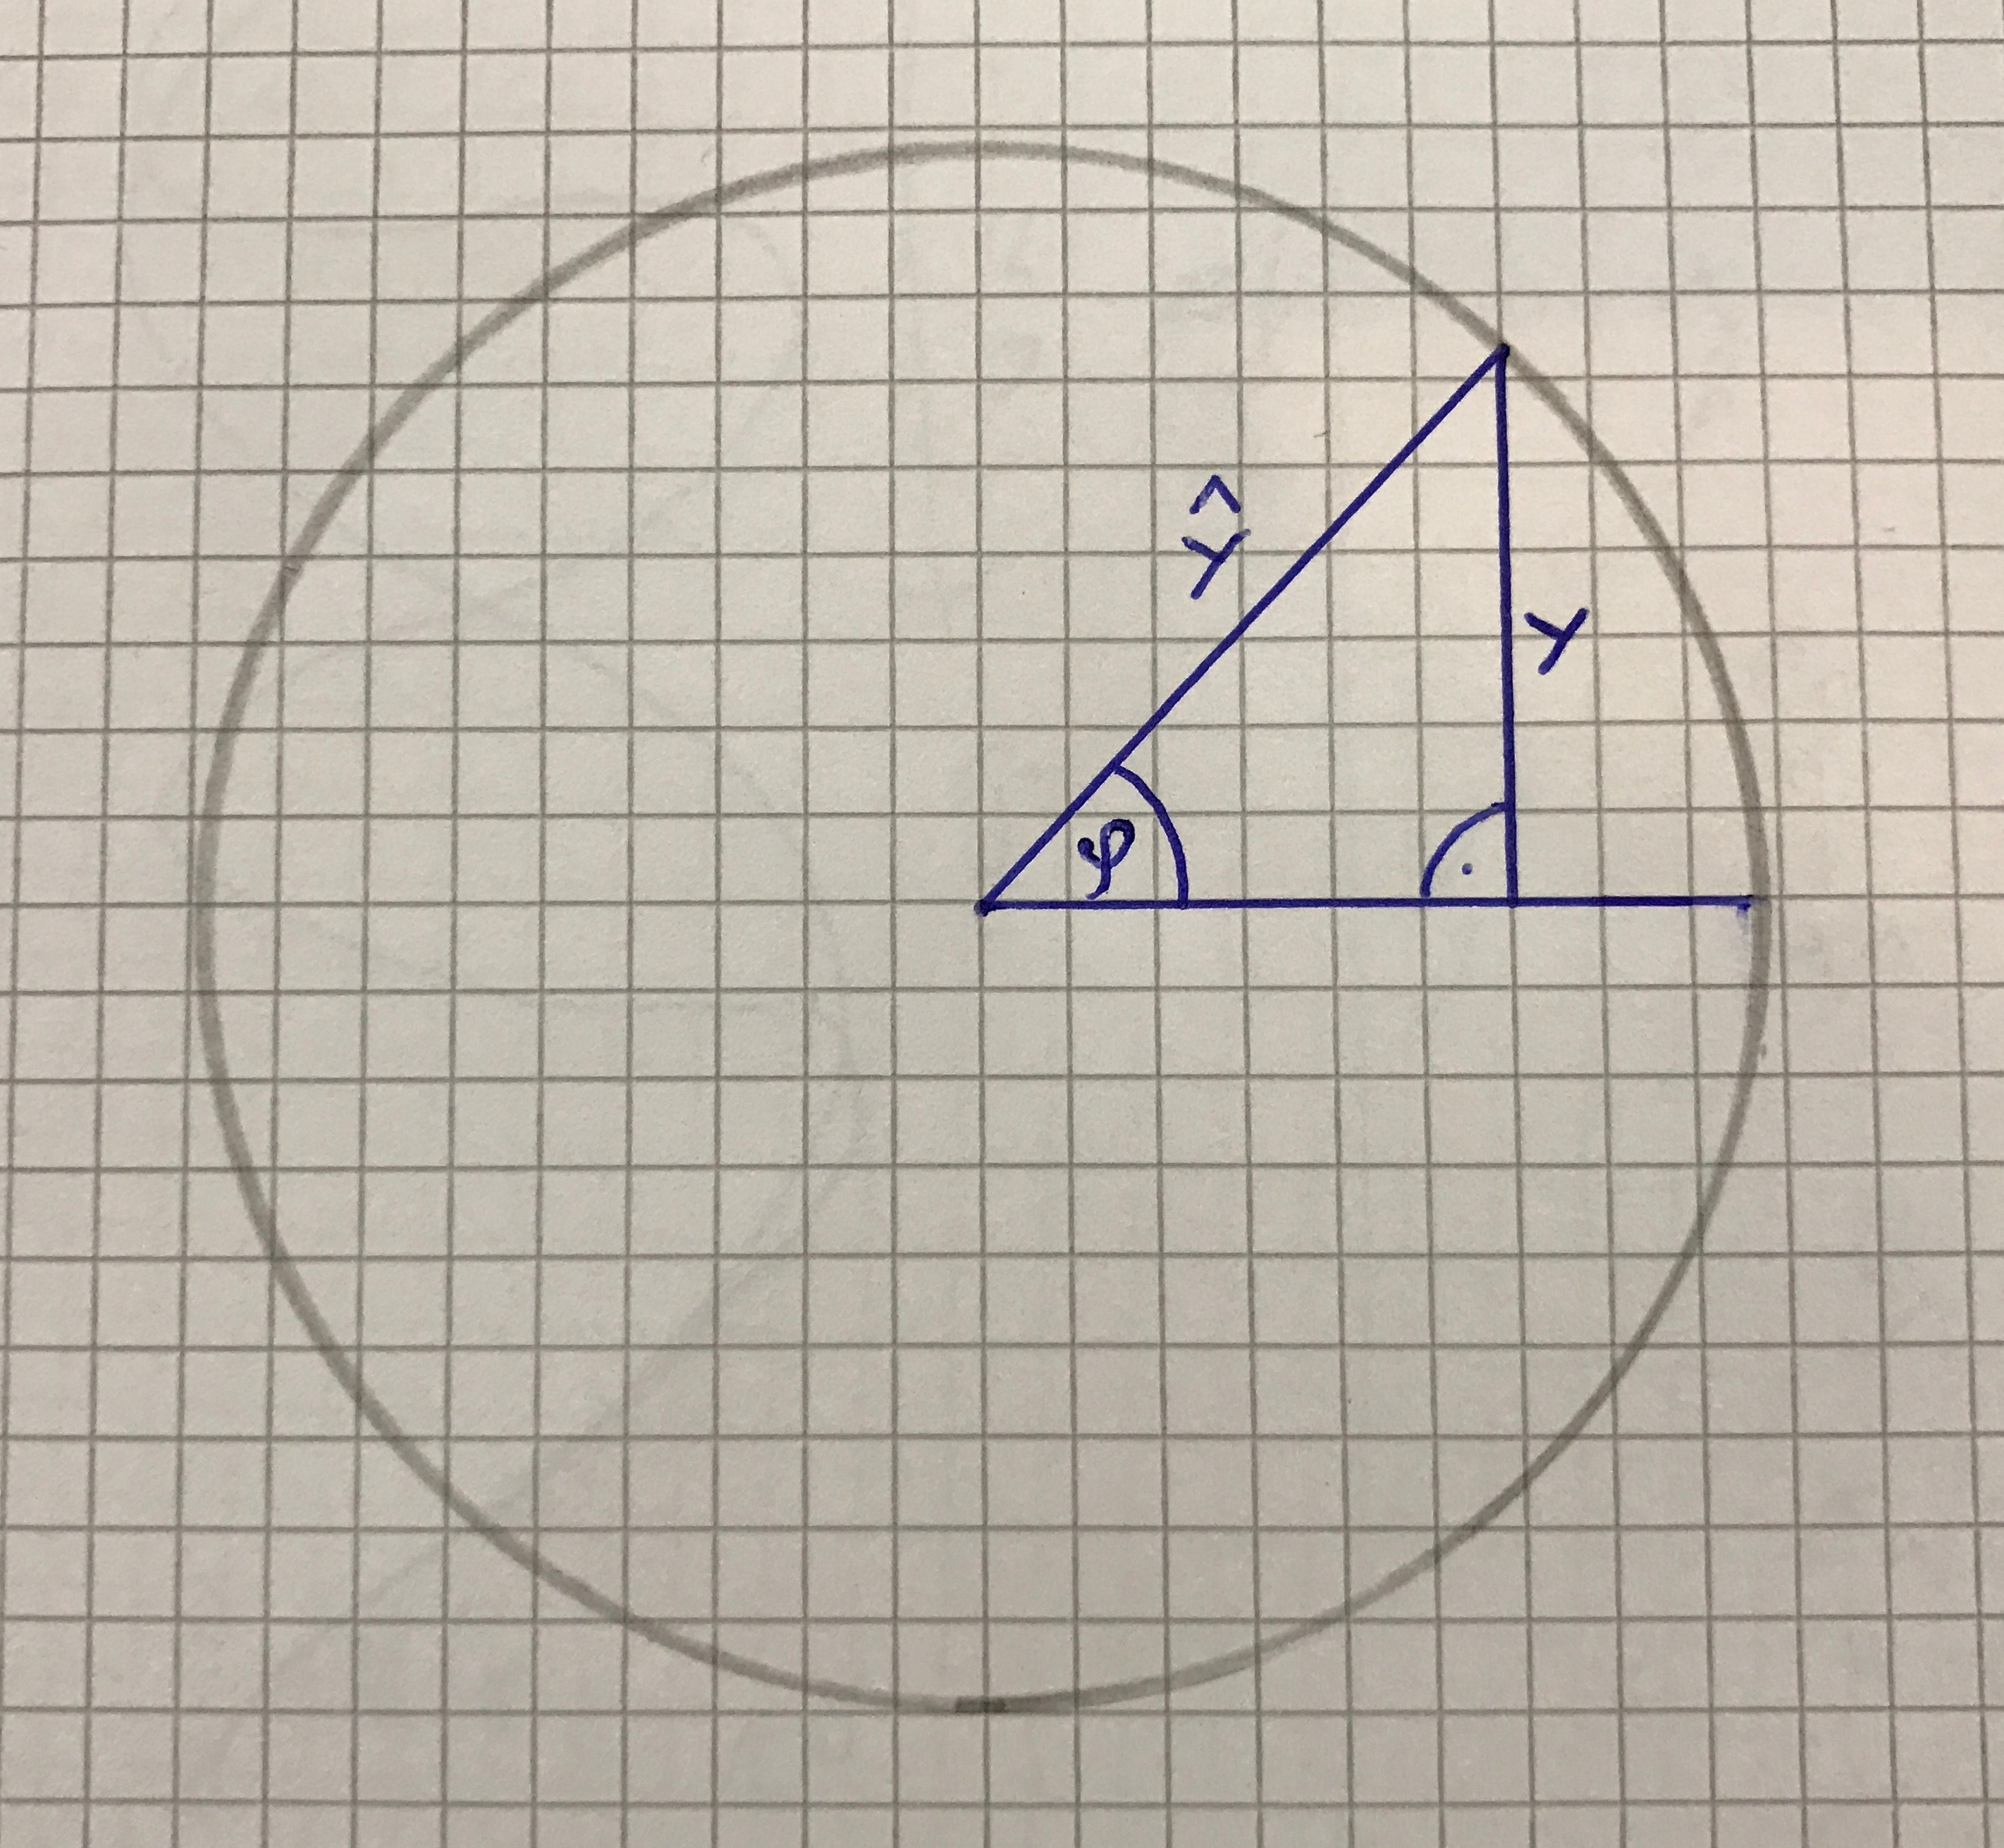
\includegraphics[width=0.48\textwidth]{img/welle_zeigerdarstellung.jpg}
				\caption{Die Elongation bei dem Phasenwinkel $\varphi$}
				\label{img:welle_zeigerdarstellung}
			\end{figure}
		
		
			\noindent Die Wellengleichung \ref{einfache_wellengleichung} muss nun um $\varphi_0$ erweitert werden, da an einem anderen Ort eine Phasenverschiebung herrscht:
		
			\begin{equation}\label{wellengleichung_phi0}
				y=\hat{y}\cdot sin\left(\frac{2\pi}{T}\cdot t + \varphi_0\right)
			\end{equation}			
			Betrachtet man nun nicht den Ort $x_0 = 0$ sondern $x_0=x$, setzt die Welle erst später ein, da die Strecke $x$ erst zurückgelegt werden muss. Genauso gut kann man sagen, dass $\varphi=\frac{2\pi}{T}\cdot t + \varphi_0=0$ gilt, wenn die Welle den Ort $x_0=x$ erreicht, also zum Zeitpunkt 
			
			\begin{equation}
				t=\frac{x}{c} = \frac{x}{\frac{\lambda}{T}}=\frac{T\cdot x}{\lambda}
			\end{equation}
			Damit ist der Winkel $\varphi$ zum Ankunftszeitpunkt 
			
			\begin{equation}\label{wellengleichung_ankunftswinkel}
				\begin{aligned}
					\frac{2\pi}{T}\cdot \frac{T\cdot x}{\lambda} + \varphi_0 &=0\\
					\varphi_0 = - \frac{2\pi}{T}\cdot \frac{T\cdot x}{\lambda}&= - 2\pi\cdot \frac{x}{\lambda}
				\end{aligned}
			\end{equation}
			Setzt man nun Gleichung \ref{wellengleichung_ankunftswinkel} in Gleichung \ref{wellengleichung_phi0} ein, erhält man die Gleichung
			
			\begin{equation}
				y(t, x)=\hat{y}\cdot sin\left(\frac{2\pi}{T}\cdot t - 2\pi\cdot \frac{x}{\lambda}\right) = \hat{y}\cdot\sin\left(2\pi\left(\frac{t}{T}-\frac{x}{\lambda} \right)\right)
			\end{equation}
			
			
		\subsection{Huygenssches Prinzip}
			Das Huygenssche Prinzip nach Christian Huygens besagt, dass jeder Punkt einer Welle als Elementarwelle, also dem Ausgangspunkt einer neuen Welle, betrachtet werden kann.
			
			\noindent Damit ist einfache Erklärung von Beugung, Brechung und Reflexion möglich.
			
				\subsubsection{Beugung}
					Beugung bzw. Diffraktion bezeichnet die Ablenkung einer Welle an einem Hindernis. So kann sich eine Welle auch in Räume ausbreiten die auf direktem Weg vom Ursprung der Welle nicht zu erreichen wären.
					
					\noindent Sichtbar wird Beugung in dem Moment in dem sich eine Wellenfront durch einen Spalt bewegt, dessen Breite sich in der Größenordnung der Wellenlänge befindet. 
					
					\begin{figure}[H]
						\centering
						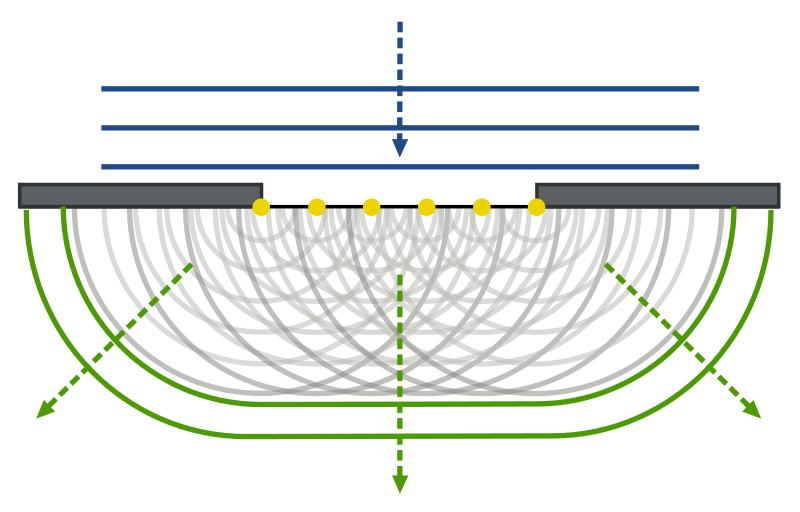
\includegraphics[width=0.5\textwidth]{img/beugung.png}
						\caption{Beugung am Einzelspalt}
						\label{img:beugung}
					\end{figure}
					
					\noindent So haben Schallwellen eine Wellenlänge die sich in der Größenordnung von z.B. einer Tür befinden, während Lichtwellen eine deutlich geringere Wellenlänge haben. Deswegen können wir um die Ecke hören, aber nicht sehen.
					
				\subsubsection{Brechung}
					Wenn an der Grenze zweier Medien eine Welle nicht senkrecht auftrifft, so ändert diese ihre Ausbreitungsrichtung. Dieses Phänomen lässt sich ebenfalls mit dem Huygensschen Prinzip erklären.
					
					\begin{itemize}
						\item Durch das schräge Auftreffen werden die Oszillatoren des zweiten Mediums zeitlich versetzt zu Schwingungen angeregt.
						\item Nach dem Huygensschen Prinzip ist jeder dieser Oszillatoren wieder der Ausgangspunkt einer neuen Elementarwelle.
						\item Die neuen Elementarwellen überlagern sich zu neuen Wellenfronten.
						\item Da die Ausbreitungsgeschwindigkeit in dem neuen Medium anders ist findet eine konstruktive Überlagerung in einem anderen Winkel als dem Auftreffwinkel statt.
					\end{itemize}
				
					\noindent Beim Medienwechsel ändert sich darüber hinaus auch die Wellenlänge, da sich die Ausbreitungsgeschwindigkeit ändert, während die Frequenz gleich bleibt.
					
					\begin{figure}[H]
						\centering
						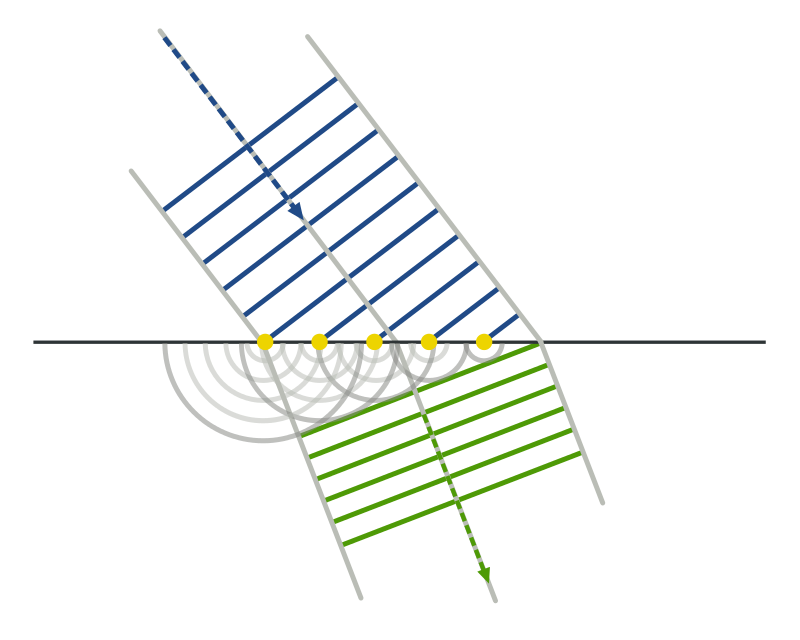
\includegraphics[width=0.5\textwidth]{img/brechung.png}
						\caption{Brechung beim Medienwechsel}
						\label{img:brechung}
					\end{figure}
				
					\noindent Dabei stehen Winkel und Geschwindigkeit im Folgenden Verhältnis zueinander, wobei $\alpha$ den Einfallswinkel, $\beta$ den Ausfallwinkel und $v_1$ und $v_2$ die Geschwindigkeiten beschreiben:
				
					\begin{equation}
						\frac{sin(\alpha)}{sin(\beta)}=\frac{v_1}{v_2}
					\end{equation}
					
				\subsubsection{Reflexion}
					Trifft eine Welle auf ein Hindernis, wird diese dort reflektiert. Betrachtet man dabei die Oszillatoren vor dem Hindernis als Ausgangspunkt neuer Elementarwellen, lässt sich die Reflexion einfach erklären. 
					
					\noindent Der Radius der neuen Elementarwellen vergrößert sich proportional zur Zeit. In Abbildung \ref{img:reflexion} sieht man wie die ersten Kreise angewachsen sind, während der aktuelle Auftreffpunkt nach rechts wandert. Durch die Überlagerung der Elementarwellen bildet sich nun eine neue Wellenfront. 
					
					\noindent Der Einfallswinkel und der Austrittswinkel sind gleich.
					
					\begin{figure}[H]
						\centering
						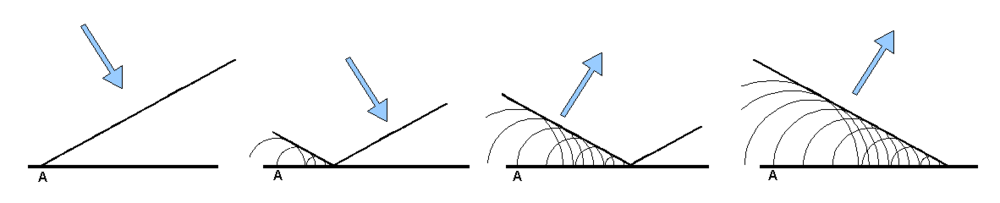
\includegraphics[width=0.9\textwidth]{img/reflexion.png}
						\caption{Reflexion einer Welle}
						\label{img:reflexion}
					\end{figure}

		\subsection{Harmonischer Oszillator}
			\begin{figure}[H]
				\centering
				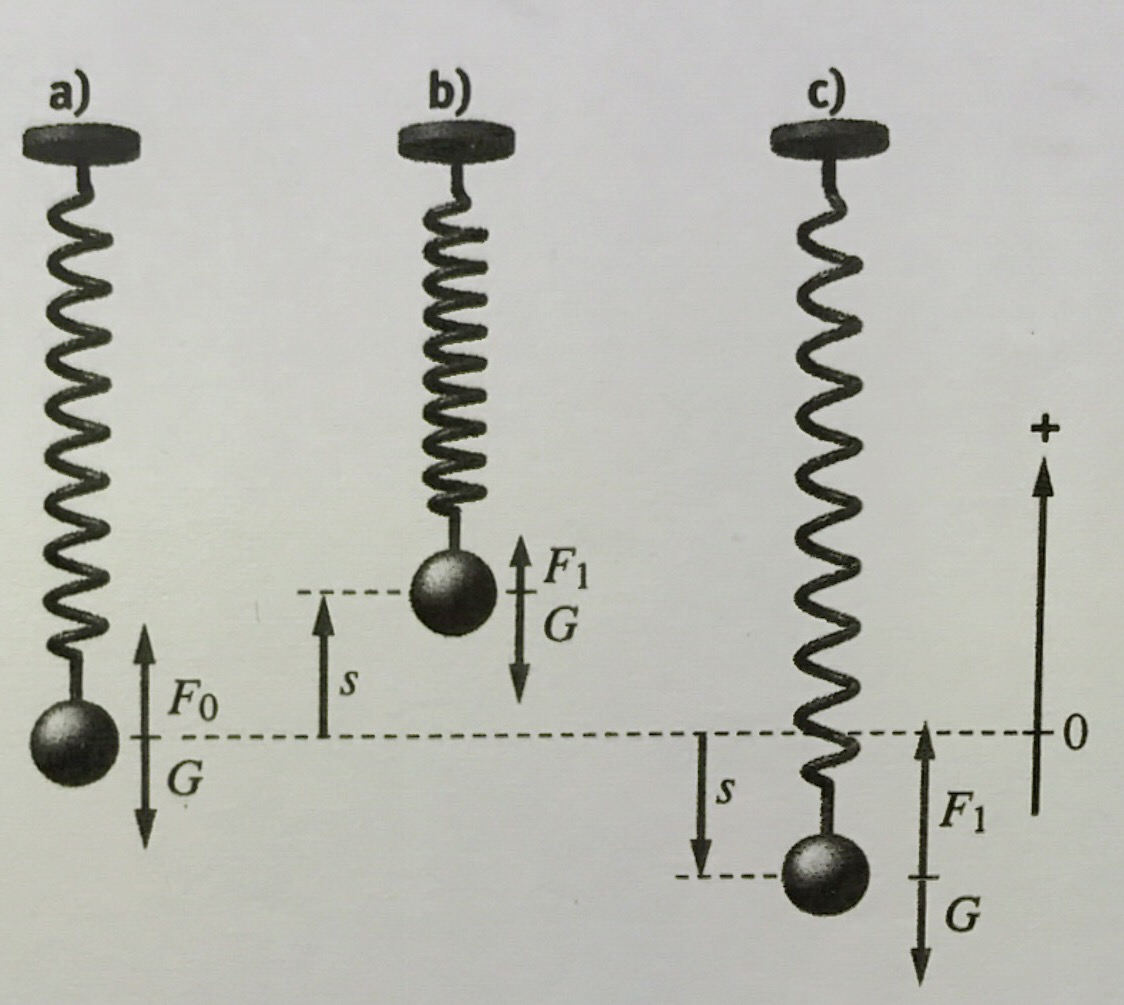
\includegraphics[width=0.48\textwidth]{img/Federpendel_001.jpg}
				\caption{Das Federpendel mit der Auslenkung $s$}
				\label{img:federpendel_001}
			\end{figure}
		

	
			In der in Abbildung \ref{img:federpendel_001}a dargestellten Gleichgewichtslage ist die nach oben gerichtete und damit positive Federkraft $F_0$ vom Betrag her genau so groß wie die nach unten gerichtete und damit negative Gewichtskraft $G$. Es gilt $G=-F_0$ und damit
			\begin{equation}
				F=G+F_0=0
			\end{equation}
			Wenn man den Körper wie in Abbildung \ref{img:federpendel_001}b zu sehen um die Strecke $s$ nach oben auslängt, wird $F_1$ kleiner: $F_1 = F_0-Ds$. Mit der Näherung, dass $G$ konstant bleibt, gilt:
			\begin{equation}
				F=G+F_1= G+F_0-Ds = -Ds
			\end{equation}
			Analog wird $F_1$ bei einer Auslenkung nach unten größer: $F_1 = F_0-Ds$. Da $s$ in Abbildung \ref{img:federpendel_001}c kleiner $0$ ist, ist $-Ds$ positiv. Damit ist auch in Fall c die resultierende Kraft
			\begin{equation}\label{harmonischer_oszillator:fds}
			F=G+F_1= G+F_0-Ds = -Ds
			\end{equation}
			Die Rückstellkraft $F$ ist also proportional zur Elongation $s$. Das negative Vorzeichen, beschreibt, dass die Kraft immer entgegen der Elongationsrichtung steht. Sie wirkt also immer zur Gleichgewichtslage.
			\begin{equation}
				F= -Ds
			\end{equation}
			Mithilfe der Beschleunigungsgleichung $a(t)=-\hat{s}\cdot\omega^2\cdot\sin\left(\omega\cdot t\right)$ und Newtons Gleichung für die Kraft (Gleichung \ref{kraft:fma}) erhalten wir:
			\begin{equation}\label{harmonischer_oszillator:fma}
				F= m\cdot a = -m\cdot \hat{s}\cdot\omega^2\cdot\sin\left(\omega\cdot t\right)
			\end{equation}
			Da $s=\hat{s} \cdot\sin(\omega\cdot t)$ gilt, können wir die Gleichung \ref{harmonischer_oszillator:fma} wie folgt vereinfachen:
			\begin{equation}
				F= m\cdot a = -m\cdot\omega^2\cdot s
			\end{equation}
			Diese können wir mit Gleichung \ref{harmonischer_oszillator:fds} gleichsetzen und erhalten:
			\begin{equation}
				-m\cdot\omega^2\cdot s = -Ds \Leftrightarrow D=m\cdot\omega^2
			\end{equation}
			Setzten wir nun $\omega=\frac{2\pi}{T}$ ein, erhalten wir eine Formel für die Periodendauer T:
			\begin{equation}
				T=2\pi\cdot\sqrt{\frac{m}{D}}
			\end{equation}
	
		\subsection{Fadenpendel}
		
			\begin{figure}[H]
				\centering
				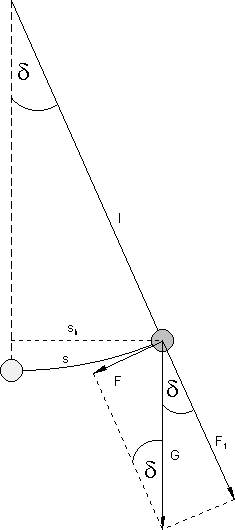
\includegraphics[width=0.2\textwidth]{img/fadenpend02_mechanschwing_gru.png}
				\caption{Skizze zum Fadenpendel}
				\label{img:fadenpend02_mechanschwing_gru}
			\end{figure}
			Beim Fadenpendel ist die Rückstellkraft parallel zur Tangente des Schwingkreises. Damit steht sie senkrecht auf dem Seil, an dem die schwingende Masse befestigt ist. Damit gilt
			
			\begin{equation}
			\begin{aligned}
					F &= G \cdot sin(\delta)\\
					&= m \cdot g \cdot sin(\delta)\\
					&= m \cdot g \cdot sin(\frac{s}{l})
				\end{aligned}
			\end{equation}
			Wenn man nun die Vereinfachung annimmt, dass die direkte Entfernung zur Gleichgewichtslage $s_h$ gleich der Entfernung auf dem Schwingkreises $s$ \textit{bei kleinen Werten für $\delta$ ist}, dann ist $\sin(\delta) = \frac{s_h}{l} \approx \frac{s}{l}$:
			
			\begin{equation}
					F = m \cdot g \cdot \frac{s}{l} = s \cdot \frac{m \cdot g}{l}
			\end{equation}
			Damit ist $F$ proportional zu $s$ und das lineare Kraftgesetz $F=-DS$ mit $D=\frac{m \cdot g}{l}$ kann angewendet werden. Nun lässt sich die Periodendauer folgendermaßen bestimmen:
			\begin{equation}
				\begin{aligned}
					T&=2\pi\cdot\sqrt{\frac{m}{D}}\\
					&=2\pi\cdot\sqrt{\frac{m}{\frac{m \cdot g}{l}}}\\
					&=2\pi\cdot\sqrt{\frac{l}{g}}
				\end{aligned}
			\end{equation}
			
		
		\subsection{Doppelspalt}
			
			Am Doppelspalt werden Interferenzmuster von zwei gleichen, in Phase schwingenden Wellen gezeigt. Dafür wird vor dem Doppelspalt eine Welle erzeugt, welche dann auf ein Hindernis mit zwei Spalten trifft. Deren Breite sollte sich in der Größenordnung der Wellenlänge der Welle befinden. Dadurch erhält man zwei Elementarwellen, die sich kreisförmig ausbreiten, die die gleiche Frequenz haben und die in Phase miteinander schwingen. Diese beiden neuen Wellen erzeugen dann ein Interferenzmuster welches zum Beispiel auf einer geraden oder gekrümmten Projektionsfläche betrachtet werden kann.
			
			\begin{figure}[H]
				\centering
				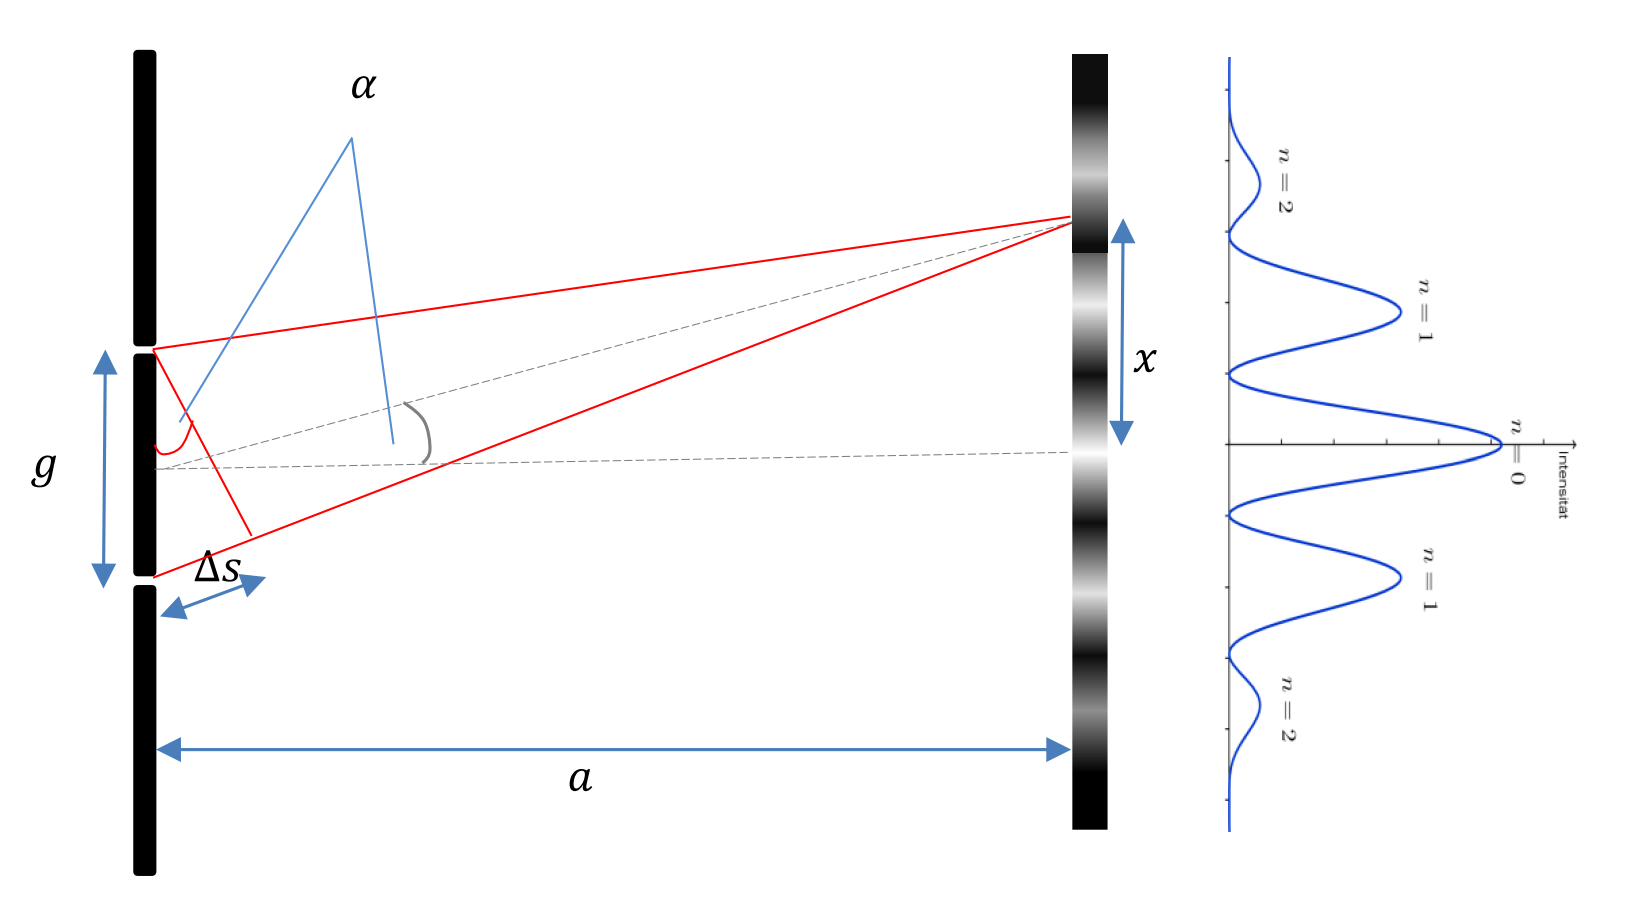
\includegraphics[width=0.5\textwidth]{img/Inteferenz_am_Doppelspalt.png}
				\label{img:inteferenz_am_doppelspalt}
				\caption{Darstellung der Interferenz am Doppelspalt auf einer geraden Projektionsfläche}
			\end{figure}
			$\delta s$ ist die Wellenlänge, wenn $s1$ und $s2$ je die Distanz von den Spalten zum ersten Maximum ist. Entsprechend gilt $\frac{\delta s}{n}$ für das $n$-te Maximum. Mithilfe von Pythagoras ($a^2+b^2=c^2$) lässt sich dann folgende Gleichung für die Wellenlänge berechnen, vorausgesetzt es sind einige Werte gegeben:
				
			\begin{equation}
				\begin{aligned}
					\frac{\delta s}{n} &= \lambda
					&= \frac{\abs{\sqrt{l^2 + \left(x - \frac{g}{2} \right)^2} - \sqrt{l^2 + \left(x + \frac{g}{2} \right)^2}}}{n}
				\end{aligned}
			\end{equation}
			
			
		\subsection{Überlagerung von harmonischen Schwingungen}
	
			\subsubsection{Überlagerung gleicher Frequenzen}
			
				Überlagert man zwei Schwingungen mit gleicher Frequenz erhält man wieder eine harmonische Schwingung mit derselben Frequenz. Phase und Amplitude ergeben sich aus vektorieller Addition. Es kommt bei Phasengleichheit zur konstruktiven Interferenz, bei einer Phasendifferenz von $\pi$ zur destruktiven Interferenz.
			
			\subsubsection{Überlagerung unterschiedlicher Frequenzen und Schwebung}
			
				Überlagert man zwei Schwingungen mit unterschiedlichen Frequenzen $f_1$ und $f_2$ überlagern sie sich zu einer Schwebung. Es entsteht deshalb auch \textit{keine} harmonische Schwingung. Die neue Schwingung hat die Grundfrequenz
				
				\begin{equation}
					f=\frac{f_1+f_2}{2}
				\end{equation}
				die Schwebungsfrequenz
				
				\begin{equation}
					f_s=|f_1-f_2|
				\end{equation}
				und die Modulationsfrequenz
				
				\begin{equation}
				f_{mod}=\frac{|f_1-f_2|}{2}
				\end{equation}
				
				\begin{figure}[H]
					\centering
					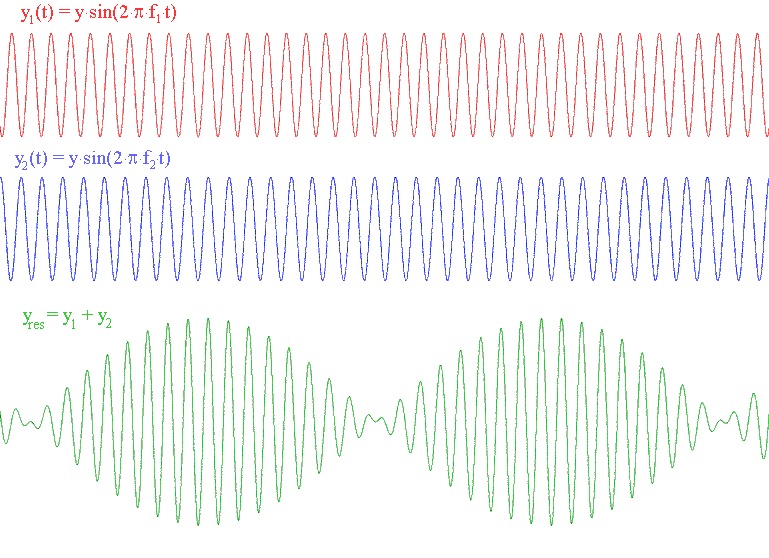
\includegraphics[width=0.5\textwidth]{img/schwebung_k_akustwellen_gru.png}
					\label{img:schwebung_k_akustwellen_gru}
					\caption{Visualisierung der Schwebung}
				\end{figure}
			
		\subsection{Akustische Unschärfe}%TODO: Einbauen: Akustische Unschärfe
	
		\subsection{Dopplereffekt}
		
			Wenn der Empfänger oder der Sender sich bewegt, kommt es zum Dopplereffekt.
			
			
			\subsubsection{Bewegter Sender}
			
				Für den Empfänger ändert sich die Wellenlänge, dagegen bleibt die Ausbreitungsgeschwindigkeit konstant. Bewegt sich der Sender um $\Delta s = v_S\cdot T$, dann ist die neue Wellenlänge beim Annähren $\lambda - v_S\cdot T$ und beim Entfernen $\lambda + v_S\cdot T$. Für die wahrgenommene Frequenz ergibt sich dann:
				
				\begin{equation}
				\begin{aligned} 
					f'&=\frac{c}{\lambda \mp v_S\cdot T} \\
					&= \frac{c}{\frac{c}{f_0} \mp v_S\cdot T}\\
					&= f_0\cdot\frac{c}{c \mp v_S\cdot T\cdot f_0}\\
					&= f_0\cdot\frac{c}{c \mp v_S\cdot T\cdot \frac{1}{T}}\\
					&= f_0\cdot\frac{1}{1 \mp \frac{v_S}{c}}
				\end{aligned}
				\end{equation}
				
			\subsubsection{Bewegter Empfänger}
				Hat man dagegen einen bewegten Empfänger ändert sich die Ausbreitungsgeschwindigkeit und die Wellenlänge bleibt erhalten. Bewegt sich der Empfänger mit der Geschwindigkeit $v_E$, dann ist die Geschwindigkeit der Welle beim nähren $c+v_E$ und beim entfernen $c-v_E$. Für die wahrgenommene Frequenz ergibt sich dann:
				
				\begin{equation}
					f' = \frac{c \pm v_E}{\lambda} =  \frac{c \pm v_E}{\frac{c}{f_0}} = f_0\cdot\frac{c\pm v_E}{c} = f_0\cdot\left(1\pm \frac{v_E}{c}\right)
				\end{equation}
				
			\subsubsection{Bewegter Sender und Empfänger}
				Bewegt sich sowohl der Sender als auch der Empfänger überlagern sich die beiden Effekte. Die resultierende Frequenz $f'$ ist dann
				
				\begin{equation}
					f' = f_0\cdot\frac{c \pm v_E}{c \mp v_S}
				\end{equation}
			
		
		\subsection{Stehende Wellen}
		
			\subsubsection{Reflexion am festen Ende}
				Das feste Ende befindet sich immer in der Ruhelage, es ist ein Schwingungsknoten. Ein ankommender Wellenberg muss ausgeglichen werden. Daraus ergibt sich, dass die zurückkommende Welle immer die horizontal gespiegelte Welle ist ($y_2 = -y_1$). Das bedeutet, dass an einem festen Ende ein Phasensprung mit $\Delta\varphi=\pi=180\si{\degree}$ stattfindet.\\
				Überlagern sich beide Wellen kommt es zu einer stehenden Welle. Sie hat Schwingungsknoten im Abstand von $n\cdot \frac{\lambda}{2}; n\in\mathbb{N}$ von der Wand.
			
			\subsubsection{Reflexion am losen Ende}
			    Da beim losen Ende die Welle nicht beeinflusst wird, gibt es keinen Phasensprung. Die Welle läuft einfach weiter nur in diesmal in die entgegengesetzte Richtung, sodass sie mit sich selbst interferieren kann. Die daraus entstehende stehende Welle hat Schwingungsknoten im Abstand von $n\cdot \frac{\lambda}{2} + \frac{\lambda}{4}; n\in\mathbb{N}$ von der Wand.
			
				
		
		\subsection{Resonanz und Eigenschwingungen}%TODO: Einbauen: Resonanz und Eigenschwingungen
	
	
	\section{Ladungen und Felder}	
		\subsection{Gravitationsfelder}
			\subsubsection{Keplersche Gesetze}
	
				\begin{enumerate}
					\item Die Planeten bewegen sich auf Ellipsen, in deren einem Brennpunkt die Sonne steht.
					\item Der von der Sonne zum Planeten gezogene Radiusvektor überstreicht in gleichen Zeiten gleiche Flächen.
					\item Die Quadrate der Umlaufzeiten der Planeten verhalten sich wie die dritte Potenz der großen Halbachsen ihrer Bahnellipsen. Das heißt $\frac{T_1^2}{T_2^2} = \frac{a_1^3}{a_2^3}$
				\end{enumerate}

			\subsubsection{Gravitationskraft}
	
				\begin{equation}
					F=G\cdot\frac{m_1\cdot m_2}{r^2}
				\end{equation}
	
			\subsubsection{Feldstärke}
	
				\begin{equation}
					g=G\cdot\frac{m}{r^2}
				\end{equation}
	
		\subsection{Elektrische Felder und Ladung}
			\subsubsection{Charakteristische Größen}
			\begin{table}[H]
				\def\arraystretch{1.5}
				\begin{tabularx}{\textwidth}{|c|c|c|X|}\hline
					Größe & Einheit & Formel & Beschreibung \\\hline
					$I$ & \si{\ampere} & $I=\frac{\Delta Q}{\Delta t}$ & Die Stromstärke.\\\hline
					$Q$ & \si{\coulomb} = \si{\ampere\second} & $Q=I\cdot\Delta t$ & Die Ladung.\\\hline
					$\varphi$ & \si{\volt} & $\varphi=\frac{E_{pot}}{Q}$ & Das Potenzial.\\\hline
					$U$ & \si{\volt} & $U=\Delta\varphi=\varphi_2-\varphi_1$ & Die Spannung ist die Differenz zweier Potenziale.\\\hline
					$P$ & \si{\watt}=\si{\joule\per\second}=\si{\kg\meter\squared\per\second\cubed} & $P=\frac{\Delta E}{\Delta t}$ & Die Leisung bezeichnet die Energie, die in einer bestimmten Zeit umgesetzt wurde.\\\hline
					$\vec{E}$ & \si{\newton\per\coulomb} & $\vec{E}=\frac{\vec{F_{el}}}{Q}$ & Die elektrische Feldstärke an einem Ort des Feldes ist der Quotient aus der Kraft $\vec{F_{el}}$ auf einen Körper an diesem Ort und seiner Ladung $Q$.\\\hline
				\end{tabularx}
				\caption {Charakteristische Größen für elektrische Felder und Ladungen}
				\label{table:elektrische_felder_grossen}
			\end{table}
				
			\subsubsection{Feldlinien und Feldflächen}
				\begin{enumerate}
					\item Feldlinien stehen in jedem Punkt senkrecht auf den Feldflächen.
					\item Feldlinien beginnen auf positiv und enden auf negativ geladenen Körpern.
					\item Feldlinien durchkreuzen sich nicht gegenseitig. Feldflächen durchkreuzen sich nicht gegenseitig.
					\item Die Richtung der Feldlinien gibt in jedem Punkt die Richtung der Kraft $\vec{F}$, die auf eine positive Ladung an diesem Punkt, an.
				\end{enumerate}
		
			\subsubsection{Elektrisches Feld}\label{elektrisches_feld}
				Ein elektrisches Feld ist ein Raum, in dem auf elektrisch geladene Körper Kräfte ausgeübt werden. Jeder geladene Körper erzeugt ein elektrisches Feld.
		
				\paragraph{Homogenes Feld}
					In einem homogenen Feld verlaufen alle Feldlinien parallel zueinander. Ein solches Feld findet man im inneren eines Plattenkondensators.
					
				\paragraph{Radiales Feld}
					In einem radialen Feld verlaufen alle Feldlinien sternförmig auseinander. Ein solches Feld findet man bei einer freien, geladenen Kugel.
			
			\subsubsection{Coulomb-Kraft}
				\begin{equation}
					\vec{F_{el}}=\frac{1}{4\pi\cdot\epsilon_0\cdot\epsilon_r}\cdot\frac{Q_1\cdot Q_2}{r^2}
				\end{equation}
			
			\subsubsection{Influence}
				Influence ist idie Verschiebung beziehungsweise Trennung der Ladung eines \textit{leitenden} Körpers unter dem Einfluss einer elektrischen Kraft, die von äußeren Ladungen ausgeübt wird. Dadurch entsteht ein Plus- und ein Minuspol.
				
			\subsubsection{Polarisation}
				Bei der Polarisation sind die Elektronen in dem Körper \textit{nicht} frei beweglich. Die Atome können sich jedoch nach der äußeren Ladung ausrichten. Dadurch entstehen viele kleine Plus- und Minuspole
				
			\subsubsection{Beschleunigung im elektrischen Feld}
				Wird eine Körper mit der Ladung $Q$ in einem elektrischen Feld mit der Spannung $U$ beschleunigt, erhält der Körper
				
				\begin{equation}
					E_{kin} = Q\cdot U
				\end{equation}
				Für ein Elektron gilt also
				\begin{equation}\label{elektrisches_feld:beschleunigung_elektron}
					E_{kin} = e\cdot U
				\end{equation}
			
			
			\subsubsection{Plattenkondensator}
				Mithilfe der Definition der elektrischen Feldstärke $\vec{F}=Q\cdot\vec{E}$ und der Gleichung \ref{energie:fs} erhält man:
			
				\begin{equation}
					E=\vec{F}\cdot d = Q\cdot\vec{E}\cdot d
				\end{equation}
				Setzt man dies nun in die Gleichung $U=\frac{E}{Q}$ ein kann man die elektrische Feldstärke eines Plattenkondensators $\vec{E}$ wie folgt berechnen:
				
				\begin{equation}\label{plattenkondensator:e}
					\vec{E}=\frac{U}{d}
				\end{equation}
	
			\subsubsection{Anwendungen}
		
				\paragraph{Elektrische Feldstärke}
					Um die elektrische Feldstärke zu ermitteln, kann man wie in Abbildung \ref{img:efeldwaag_ladungenober_ver} ein Ladung in ein elektrisches Feld bringen und dieses wiegen. Wenn die Ladung $Q$ und die Masse $m$ des Körpers bekannt ist, kann man mit $\vec{E}=\frac{\vec{F_{el}}}{Q}$, $\vec{F_g}=m\cdot g$ und $m_{angezeigt}=\frac{\vec{F_g} + \vec{F_{el}}}{g}$ die elektrische Feldstärke $\vec{E}$ bestimmen.
					\begin{figure}[H]
						\centering
						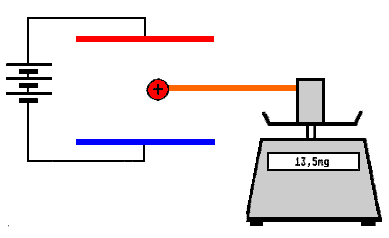
\includegraphics[width=0.5\textwidth]{img/efeldwaag_ladungenober_ver.png}
						\caption{Elektrische Feldstärke wiegen.}
						\label{img:efeldwaag_ladungenober_ver}
					\end{figure}
				
				\paragraph{Millikan-Versuch}
					
					Beim Millikanversuch werden leicht geladene Öltröpfchen in einen Plattenkondensator gegeben. Wenn man die Spannung des Kondensators so einstellt, dass die Tröpfchen schweben, gilt
					\begin{equation}\label{millikan:f_g}
						F_G=F_{el}\Leftrightarrow m\cdot g = Q\cdot \vec{E} = Q\cdot\frac{U}{d}
					\end{equation}
					Da man $m$ aufgrund der kleinen Werte nicht direkt bestimmen kann, lässt man die Öltröpfchen in dem ausgeschalteten Plattenkondensator sinken. aufgrund von Reibungskräften wird eine maximale Geschwindigkeit erreicht, mit der man dann durch die Formel $F_G=m\cdot g =F_R$ die Masse erhält.\\
					Mit Gleichung \ref{millikan:f_g} kann man die Ladung der Öltröpfchen bestimmen. Bei der Auswertung fällt auf, dass nur ganzzahlige Vielfache von $1.662\cdot 10^{-29}C$ auftreten. Das lässt darauf schließen, dass dies eine \textit{unteilbare} Elementarladung und damit die Ladung eines Elektrons sein muss.
					
				\paragraph{Elektronenstrahlröhre}
					Eine Elektronenstrahlröhre ist ein Gerät, in dem Elektronen erst beschleunigt und dann abgelenkt werden. Auf diese Weise ist es möglich zweidimensionale Bilder auf einen Schirm zu projizieren.
					\begin{figure}[H]
						\centering
						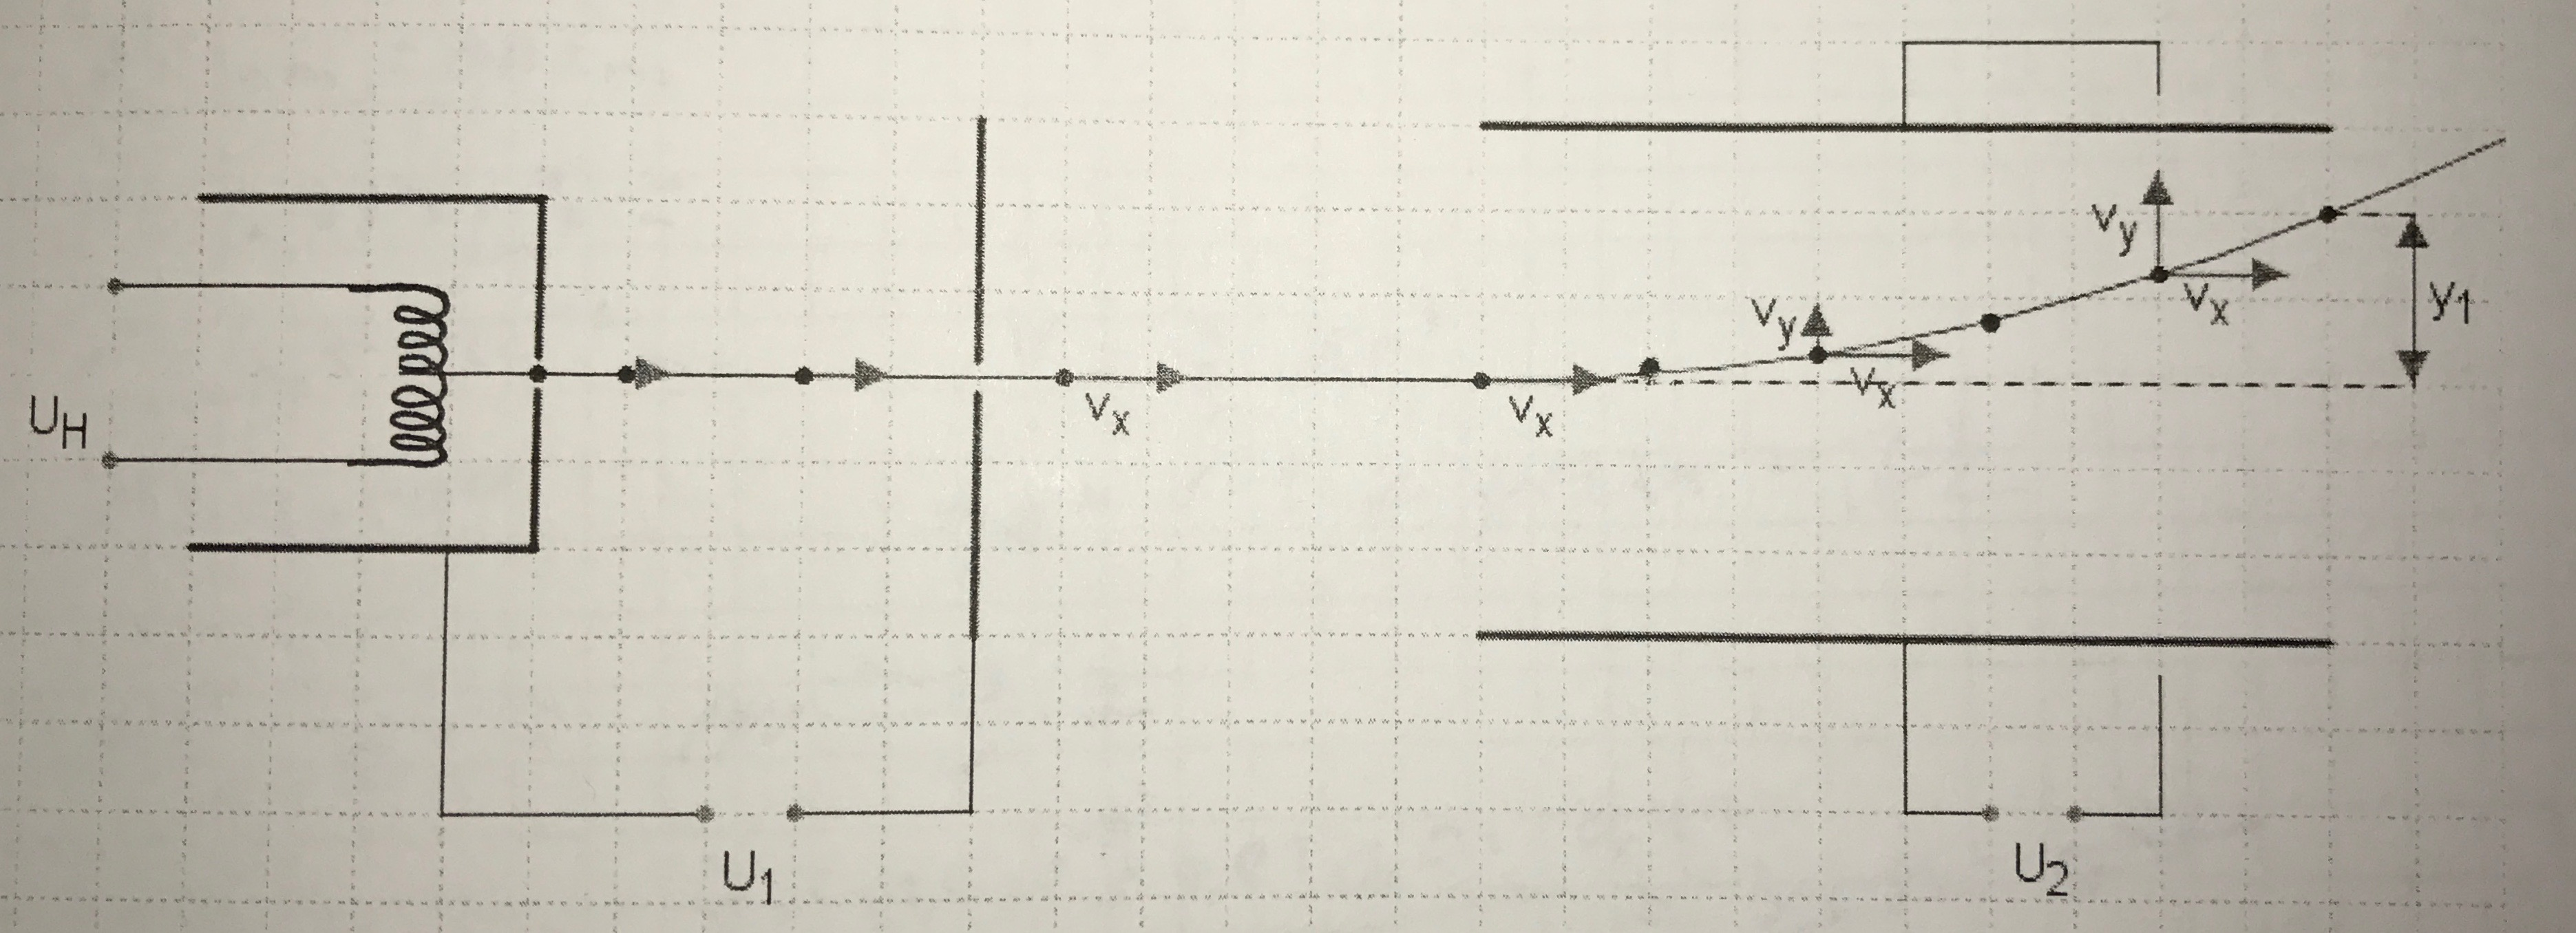
\includegraphics[width=0.8\textwidth]{img/elektronenstrahlroehre.jpg}
						\caption{Die Elektronenstrahlröhre}
						\label{img:elektronenstrahlroehre}
					\end{figure}
					\noindent Zuerst werden die Elektronen in dem ersten Plattenkondensator mit der Spannung $U_1$ beschleunigt. Dabei erhalten sich nach Gleichung  \ref{energie_kin_eq} und \ref{elektrisches_feld:beschleunigung_elektron} folgende Geschwindigkeit in x-Richtung:
					
					\begin{equation}
						\frac{1}{2}\cdot m_e \cdot v_x^2 = e \cdot U_1 \Leftrightarrow v_x = \sqrt{\frac{2\cdot e\cdot U_1}{m_e}}
					\end{equation}
					Die x-Geschwindigkeit ändert sich im zweiten Plattenkondensator mit dem Plattenabstand $d$ und der Länge $l$ nicht mehr, da hier nur eine Kraft in y-Richtung wirkt.\\
					Das Elektron braucht nach dem Bewegungsgesetzen der Mechanik folgende Zeit um den zweiten Plattenkondensator zu durchlaufen:
					
					\begin{equation}
						t=\frac{l}{v_x}\Leftrightarrow t=\frac{l}{\sqrt{\frac{2\cdot e\cdot U_1}{m_e}}}
					\end{equation}
					Setzt man  $\vec{E}=\frac{\vec{F_{el}}}{Q}$ mit $\vec{E}=\frac{U}{d}$ (Gleichung \ref{plattenkondensator:e}) gleich, erhält man
					
					\begin{equation}
						\vec{F_{el}} = \frac{U_2}{d}\cdot e
					\end{equation}
					Mit Newtons Gleichung $F=m\cdot a$ kann man die Beschleunigung in y-Richtung im zweiten Plattenkondensator berechnen:
					
					\begin{equation}
						a = \frac{U_2\cdot e}{d\cdot m_e}
					\end{equation}
					Die Ablenkung $y_1$ im zweiten Kondensator ist dann:
					
					\begin{equation}
						y_1 = \frac{1}{2}\cdot a \cdot t^2 = \frac{1}{2}\cdot \frac{U_2\cdot e}{d\cdot m_e} \cdot \frac{l^2}{\frac{2\cdot e\cdot U_1}{m_e}}=\frac{U_2\cdot l^2}{4\cdot U_1\cdot d}
					\end{equation}
					
					Die Geschwindigkeit $v_y$ beträgt nach dem zweiten Kondensator:
					
					\begin{equation}
						v_y = a\cdot t = \frac{U_2\cdot e}{d\cdot m_e} \cdot \frac{l}{\sqrt{\frac{2\cdot e\cdot U_1}{m_e}}}
					\end{equation}
					
					
	
		\subsection{Magnetische Felder}
		
			\subsubsection{Charakteristische Größen}
			\begin{table}[H]
				\def\arraystretch{1.5}
				\begin{tabularx}{\textwidth}{|c|c|c|X|}\hline
					Größe & Einheit & Formel & Beschreibung \\\hline
					$I$ & \si{\ampere} & $I=\frac{\Delta Q}{\Delta t}$ & Die Stromstärke.\\\hline
					$\vec{B}$ & \si{\newton\per\ampere\per\meter}=\si{\tesla} & $B=\frac{F_L}{I\cdot l}$ & Die magnetische Feldstärke oder Flussdichte an einem Ort des Feldes ist der Quotient aus der Kraft $\vec{F}$ auf einen Stromfluss mit der Stromstärke $I$ und der Länge $l$.\\\hline
				\end{tabularx}
				\caption {Charakteristische Größen für magnetische Felder}
				\label{table:magnetische_felder_grossen}
			\end{table}
		
			\subsubsection{Feldlinien}
				\begin{enumerate}
					\item Feldlinien beginnen am Nordpol und enden am Südpol.
					\item Feldlinien durchkreuzen sich nicht gegenseitig.
				\end{enumerate}
			
			\subsubsection{Magnetisches Feld}
				Analog zum elektrischen Feld, wie es in Abschnitt \ref{elektrisches_feld} definiert wurde, gilt: Ein magnetisches Feld ist ein Raum, in dem auf bewegte Ladungen Kräfte ausgeübt werden. Jeder bewegte Ladungen erzeugt ein magnetisches Feld.
				
				\paragraph{Homogenes Feld}
					In einem homogenen Feld verlaufen alle Feldlinien parallel zueinander. Ein solches Feld findet man im inneren eines Hufeisenmagneten, einer stromdurchflossenen Spule oder zwischen zwei Spulen (Helmholz-Spulenpaar).
					
			\subsubsection{Lorenz-Kraft}
			
				\begin{equation}
					F_L=B\cdot I \cdot l = B\cdot Q \cdot \frac{l}{t} = B\cdot Q \cdot v
				\end{equation}
				Die Lorenzkraft ist sowohl senkrecht zu den Feldlinien und damit zu $\vec{B}$ als auch zu der Geschwindigkeit $\vec{v}$: 
				\begin{equation}
					\vec{F}=Q\cdot \vec{B}\times\vec{v}
				\end{equation}
				Wenn man nicht mit Vektoren rechnet, kann man folgende Gleichung verwenden:
				\begin{equation}
				F=Q\cdot B\cdot v \cdot \sin(\alpha)
				\end{equation}
				Für ein positive Ladung kann man die Drei-Finger- oder Rechte-Hand-Regel verwenden. Dabei steht der Daumen für die Richtung der Ladungsbewegung, der Zeigefinger für die magnetische Feldstärke und der Mittelfinger für die resultierende Lorenz-Kraft.\
				
				
		\subsubsection{Halleffekt}
		
			\begin{figure}[H]
				\centering
				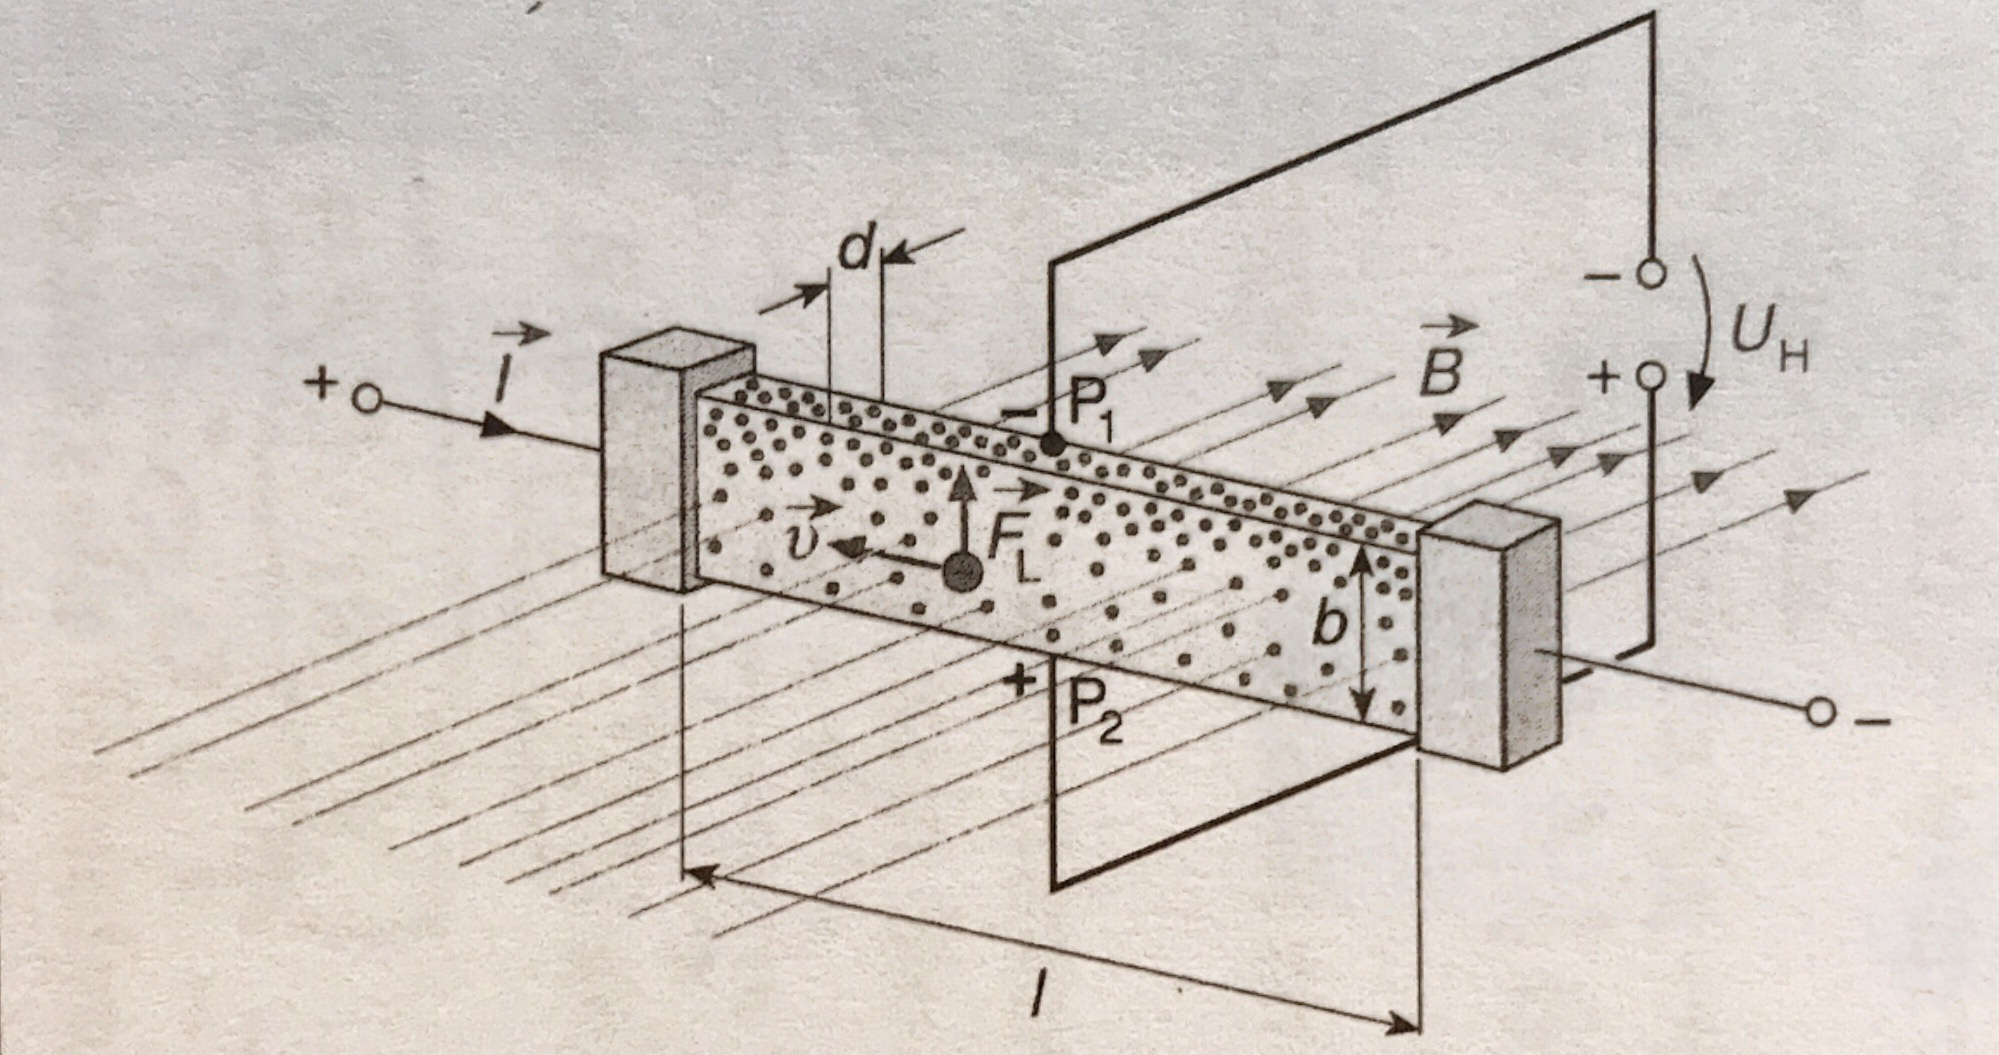
\includegraphics[width=0.5\textwidth]{img/halleffekt.jpg}
				\caption{Der Halleffekt (Schematisch)}
				\label{img:halleffekt}
			\end{figure}
		
			Die Hallspannung entsteht, wenn sich ein stromdurchflossener Leiter in einem Magnetfeld befindet (vergleiche Abbildung \ref{img:halleffekt}). Auf die bewegten Ladungen wirkt nun die Lorenzkraft. Dadurch sammeln sich auf der einen Seite des Leiters viele Elektronen. Durch die Verschiebung entsteht in dem Leiter ein elektrisches Feld, dass entgegen der Lorenzkraft wirkt. Erst wenn $\vec{F_L} = -\vec{F_{el}}$  beziehungsweise $F_L = F_{el}$ erfüllt ist, erreicht man die konstante Hallspannung $U_H$, die an dem Leiter messbar ist:
			
			\begin{equation}\label{Halleffekt:uh_short}
				\begin{aligned}
					F_L &= F_{el}\\
					Q\cdot v\cdot B &= \frac{U_H}{b}\cdot Q\\
					v\cdot B &= \frac{U_H}{b}\\
					U_H &= v\cdot B \cdot b
				\end{aligned}
			\end{equation}
			Bei einer Elektronendichte $n$ und einem Leitervolumen $V=b\cdot d\cdot l$, kann man die Stromstärke folgendermaßen ausdrücken:
			\begin{equation}\label{Halleffekt:v}
				\begin{aligned}
					I &= \frac{\Delta Q}{\Delta t}\\
					I &= \frac{n\cdot V\cdot e}{\Delta t}\\
					I &= \frac{n\cdot b\cdot d\cdot l\cdot e}{\Delta t}\\
					I &= n\cdot b\cdot d\cdot e\cdot v\\
					v &= \frac{I}{n\cdot b\cdot d\cdot e}
				\end{aligned}
			\end{equation}
			Setzt man Gleichung \ref{Halleffekt:v} in Gleichung  \ref{Halleffekt:uh_short} ein, erhällt man folgende allgemeine Form:
			
			\begin{equation}\label{Halleffekt:uh}
				\begin{aligned}
				U_H &= \frac{1}{ne}\cdot \frac{IB}{d}
				\end{aligned}
			\end{equation}
			Den materialabhängigen Vorfaktor $\frac{1}{ne}$ bezeichnet man als die Hall-Konstante $R_H$.
			
		
		\subsubsection{Elektronen auf einer Kreisbahn: Das Fadenstrahlrohr}
			
				\begin{figure}[H]
					\centering
					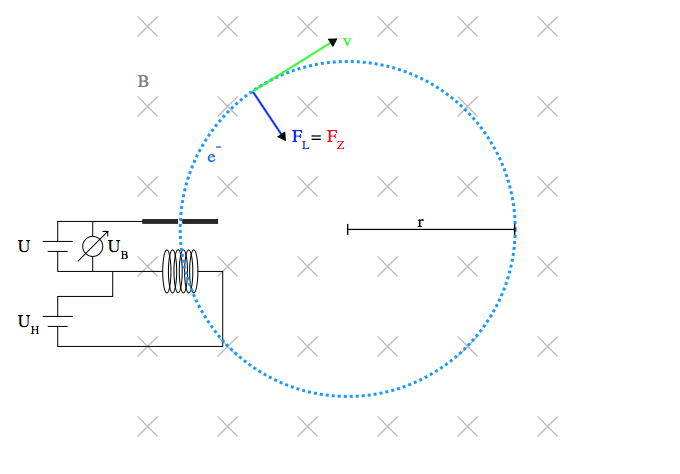
\includegraphics[width=0.5\textwidth]{img/fadensrahlrohr.png}
					\caption{Das Fadenstrahlrohr (Schematisch)}
					\label{img:fadensrahlrohr}
				\end{figure}
				Im Fadenstrahlrohr werden wie in Abbildung \ref{img:fadensrahlrohr} dargestellt Elektronen mit der Spannung $U$ beschleunigt und anschließend in ein von einem Helmholz-Spulenpaar erzeugten homogenen Magnetfeld abgelenkt. Da die Lorenzkraft \textit{immer} senkrecht zur Elektronenbewegung steht, erhalten die Elektronen nicht mehr kinetische Energie. Die Folge ist eine \textit{konstante} Geschwindigkeit auf einer Kreisbahn. Da in jeder Kreisbahn für die zum Mittelpunkt gerichtete Zentripetalkraft gilt, kann man sie mit der der zum Mittelpunkt gerichteten Lorenz-Kraft gleich setzen.
				
				\begin{equation}
				\begin{aligned} 
				F_L=B\cdot e \cdot v &= \frac{m\cdot v^2}{r} = F_Z\\
				B\cdot e &= \frac{m\cdot v}{r}\\
				\frac{e}{m} &= \frac{v}{B\cdot r}
				\end{aligned}
				\end{equation}
				Setzt man nun $e\cdot U=\frac{1}{2}\cdot m\cdot v^2$ zu $v$ umgestellt ein, erhält man folgendes:
				\begin{equation}
					\frac{e}{m} = \frac{2U}{r^2\cdot B^2}
				\end{equation}
				Historisch gesehen konnte mit dieser Formel das erste mal die Masse eines Elektrons bestimmt werden.
				
		\subsubsection{Anwendungen}
			\paragraph{Zyklotron}
			
			Das Zyklotron (vergleiche Abbildung \ref{img:aufbau_zyklotron}) besteht aus zwei D-förmigen Dosen, die von einem Magnetfeld durchsetzt werden. Zwischen den Dosen befindet sich ein elektrisches Feld, dass immer umgepolt werden muss, damit die Teilchen beschleunigt werden. Um zu ermitteln, mit welcher Frequenz die Spannung umgepolt werden muss, muss man die Lorenzkraft mit der Zentripetalkraft gleichsetzen:
			
			\begin{equation}\label{zyklotron_001}
				\begin{aligned}\
				\frac{m\cdot v_s^2}{r} &= Q \cdot v_s\cdot B\\
				\frac{m\cdot v_s}{r} &= Q \cdot B
				\end{aligned}
			\end{equation}
			
						\begin{figure}[H]
				\centering
				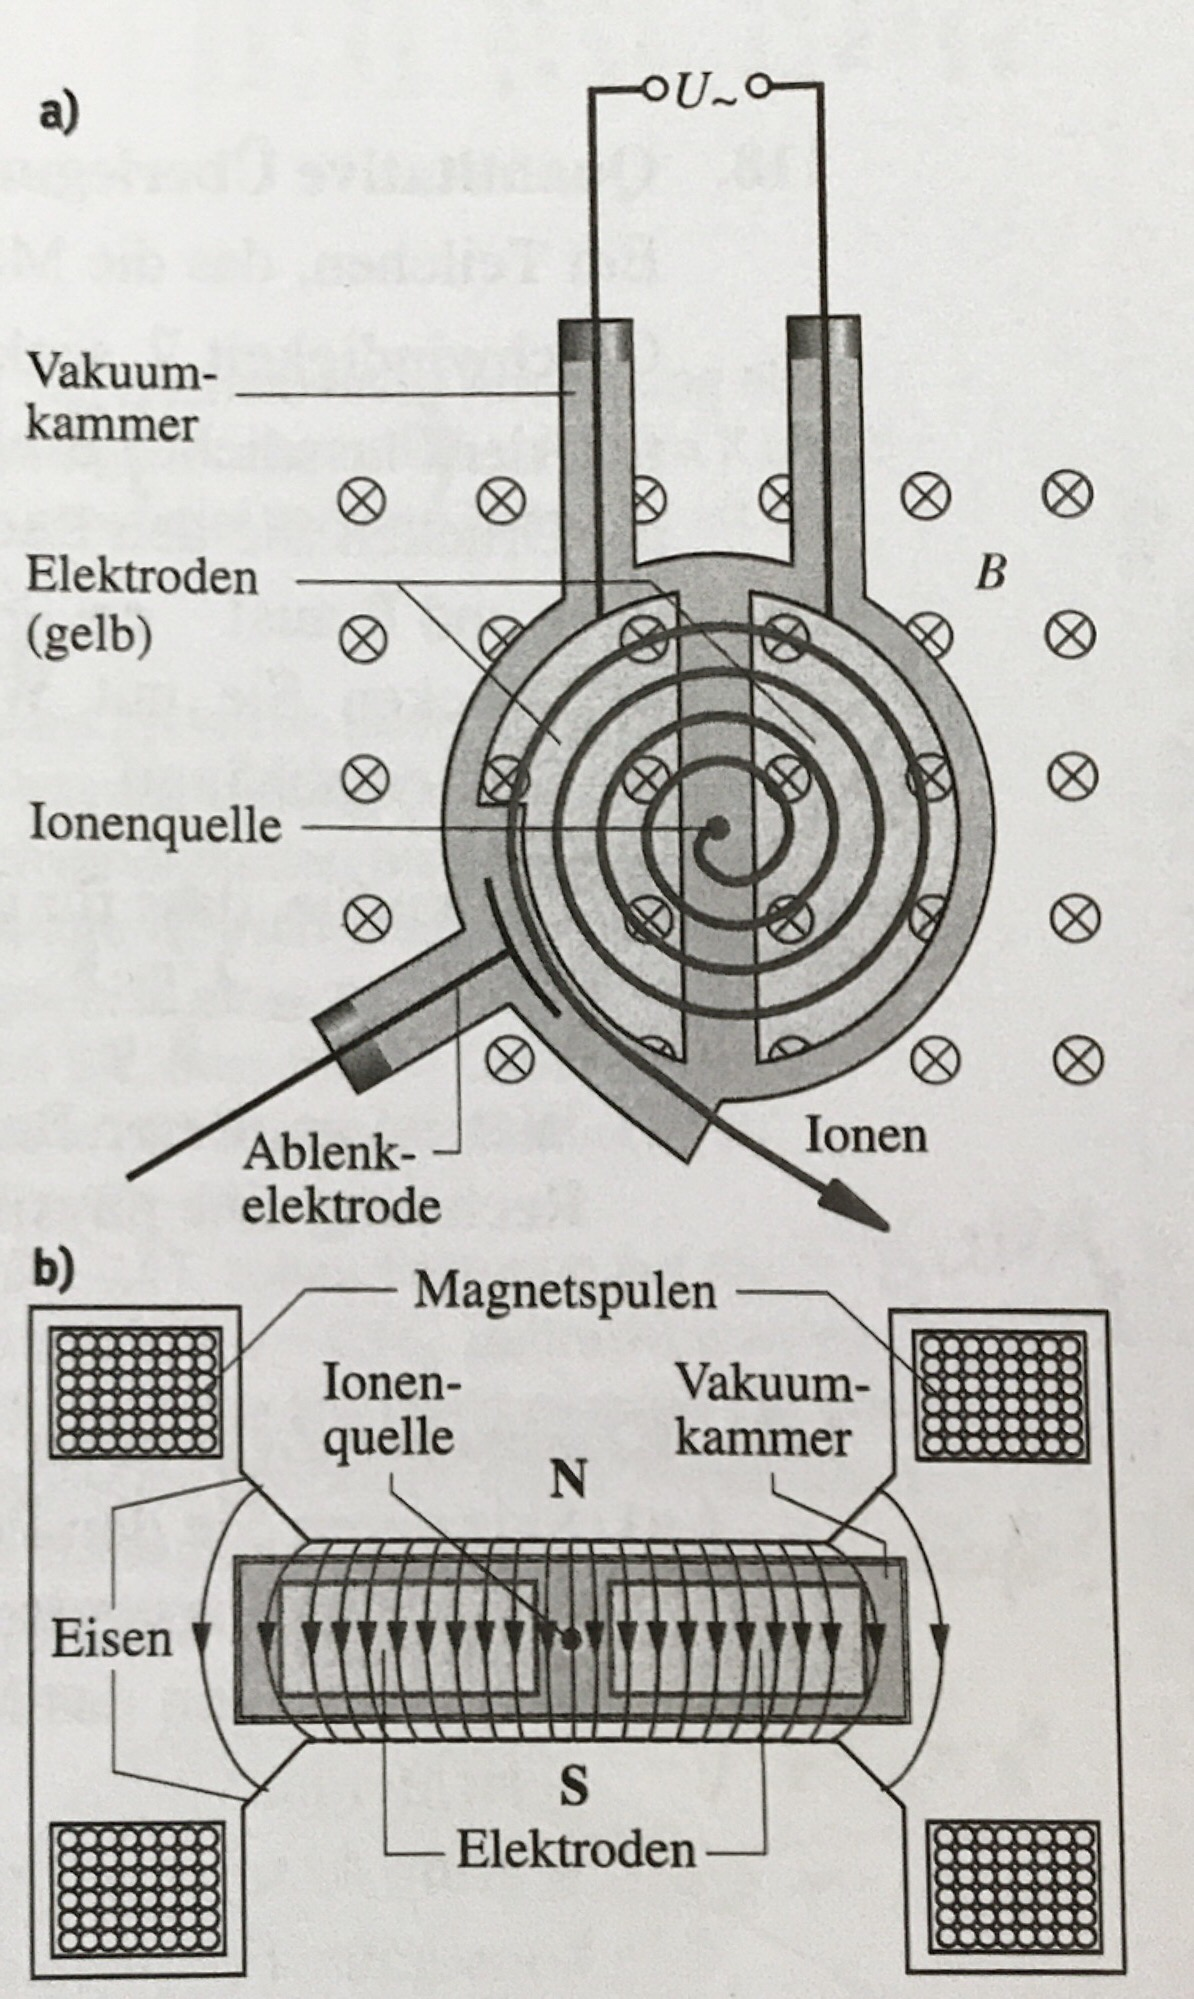
\includegraphics[width=0.3\textwidth]{img/aufbau_zyklotron.jpg}
				\caption{Das Zyklotron (Schematisch)}
				\label{img:aufbau_zyklotron}
			\end{figure}
			
			\noindent Da das Teilchen während einer vollen Periode eine Runde fliegen soll, muss die Geschwindigkeit $v_s = \frac{2\pi r}{T}$ sein. In Gleichung \ref{zyklotron_001} eingesetzt, ergibt sich folgender Zusammenhang
			
			\begin{equation}
				\begin{aligned}
				\frac{m\cdot \frac{2\pi r}{T}}{r} &= Q \cdot B\\
				m\cdot \frac{2\pi}{T} &= Q \cdot B\\
				f= \frac{1}{T} &= \frac{Q \cdot B}{2\pi\cdot m  }
				\end{aligned}
			\end{equation}
			Die Frequenz der Wechselspannung ist also unabhängig von der Geschwindigkeit, dem Bahnradius oder der Energie. Damit kann die Frequenz konstant gewählt werden und eine Beschleunigung auf kleinstem Raum wird möglich.
			

		
			
			
			\paragraph{Massenspektrometer}
				Das Massenspektrometer besteht aus zwei Teilen (siehe Abbildung \ref{img:massenspektrometer}): Dem Geschwindigkeitsfilter und dem eigentlichen Massentrenner. Es soll die Massen verschiedener geladener Teilchen bestimmen.
				
				\begin{figure}[ht]
					\centering
					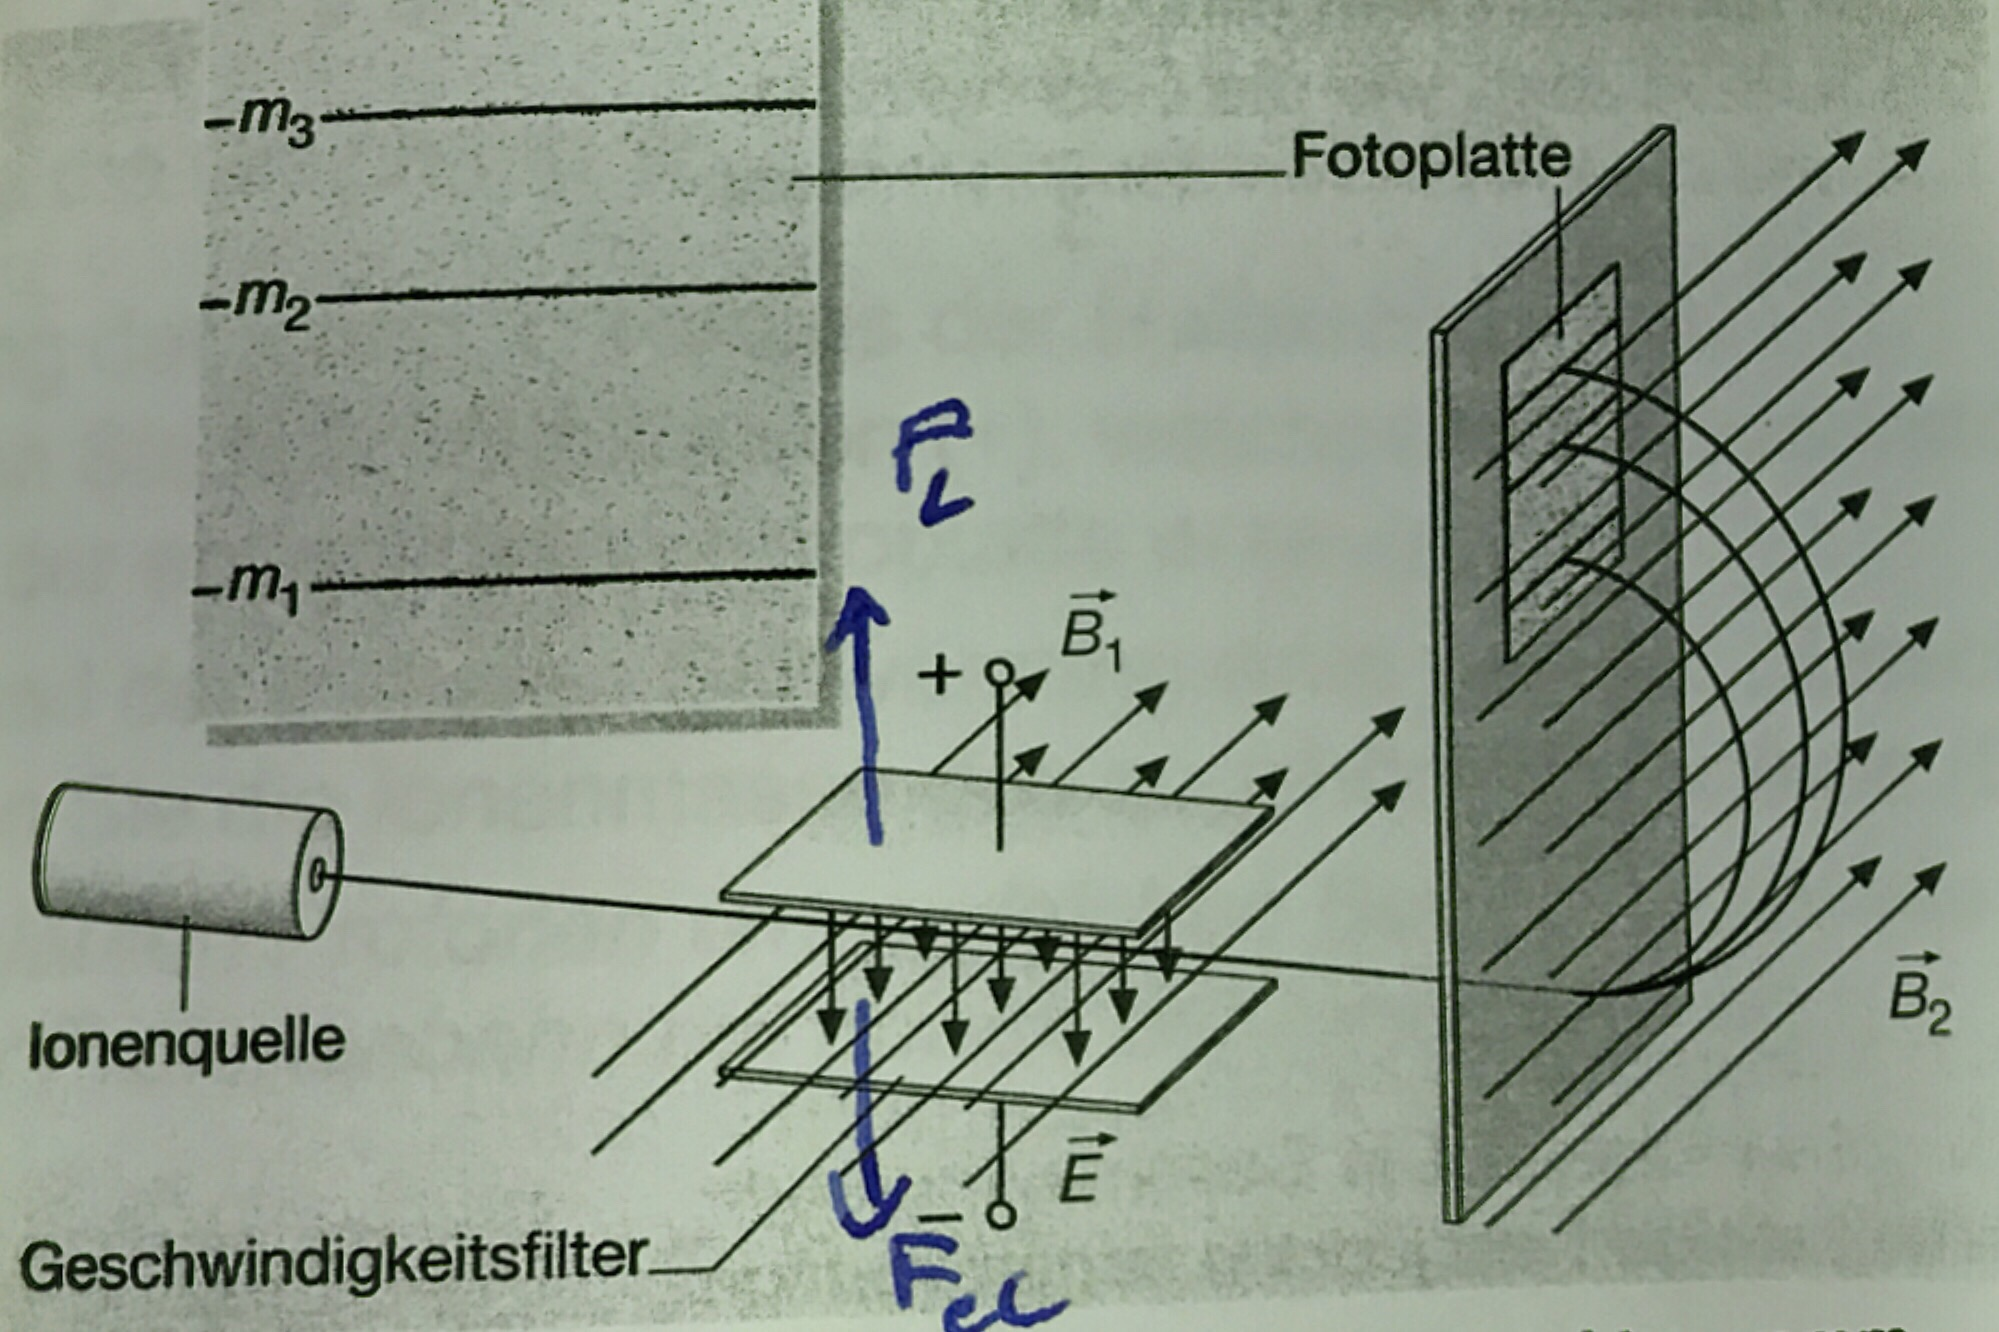
\includegraphics[width=0.5\textwidth]{img/massenspektrometer.jpg}
					\caption{Der Aufbau des Massenspektrometer (Schematisch)}
					\label{img:massenspektrometer}
				\end{figure}
				
				\subparagraph{Geschwindigkeitsfilter} Der Geschwindigkeitsfilter besteht aus zwei Feldern: Einem elektrischen mit der Feldstärke $\vec{E}$ und einem magnetischen mit der Feldstärke $\vec{B_1}$. Damit ein geladenes Teilchen den Geschwindigkeitsfilter gerade passiert und dann durch die Blende zum Massentrenner zu gelangen muss unter Vernachlässigung von Gravitation folgendes gelten:
				
				\begin{equation}
				\begin{aligned} 
					F_L&=F_{e}\\
					B\cdot Q\cdot v &= Q \cdot E\\
					v&=\frac{E}{B}
				\end{aligned}
				\end{equation}
				Es kommen also nur Teilchen mit einer spezifischen Geschwindigkeit durch den Geschwindigkeitsfilter. Alle anderen Teilchen werden entweder nach oben oder nach unten abgelenkt. Die Ladung spielt dabei keine Rolle.
				
				\subparagraph{Massentrenner} Der Massentrenner besteht aus einem homogenen Magnetfeld mit der Feldstärke $\vec{B_2}$ und einer Fotoplatte. Treten die geladenen Teilchen in dieses Magnetfeld ein, werden sie auf einer Kreisbahn abgelenkt. Es gilt:
				
				\begin{equation}
					\begin{aligned} 
						F_L=B_2\cdot Q \cdot v &= \frac{m\cdot v^2}{r} = F_Z\\
						B_2\cdot Q &= \frac{m\cdot v}{r}\\
						m&=\frac{B_2\cdot Q\cdot r}{v}
					\end{aligned}
				\end{equation}
				Da alle in das Magnetfeld eintreffenden Teilchen zuvor den Geschwindigkeitsfilter überwinden mussten, haben sie die Geschwindigkeit $v=\frac{E}{B_1}$:
				
				\begin{equation}
				\begin{aligned}
					m&=\frac{B_2\cdot Q\cdot r}{\frac{E}{B_1}}\\
					&=\frac{B_1\cdot B_2\cdot Q\cdot r}{E}
				\end{aligned}
				\end{equation}
				Die Masse der Teilchen ist also nur von den bekannten Größen $\vec{B_1}$, $\vec{B_2}$, $\vec{E}$ und $Q$ abhängig\ und lässt sich daher bestimmen.
				

				
			\paragraph{Induktion und Lenz'sche Regel}		%TODO: Einbauen: Induktion
		
	\section{Quantenphysik des Lichtes}
		\subsection{Lichtelektrischer Effekt (Photoeffekt)}
			Unter dem Photoeffekt fasst man drei unterschiedliche Effekte zusammen:
			\subsubsection{Äußerer Photoeffekt}
			
				Beobachtungen:
				\begin{enumerate}
					\item Licht kann Elektronen aus einer Metallplatte herauslösen
					\item Nur hochfrequentes (kurzwelliges) UV-Licht ist in der Lage Elektronen aus einer Zinkplatte herauszulösen. Dagegen geschieht dies nicht bei sichtbarem Licht einer Glühlampe, auch nicht bei beliebig großer Intensität.
				\end{enumerate}
				\begin{figure}[H]
					\centering
					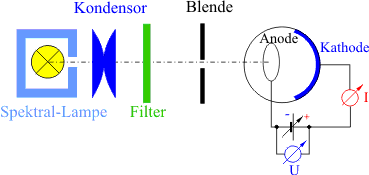
\includegraphics[width=0.5\textwidth]{img/gegenfeld03_quantenobjektp_ver.png}
					\caption{Der Aufbau der Gegenfeldmethode (Schematisch)}
					\label{img:gegenfeld03_quantenobjektp_ver}
				\end{figure}
				Diese Beobachtungen lassen sich nur mit ''Energieportionen'', den so genannten Photonen erklären. \\
				Um mehr über den Zusammenhang der Frequenz und der Energie einer Photons zu erfahren, kann man die Gegenfeldmethode (vergleiche Abbildung \ref{img:gegenfeld03_quantenobjektp_ver}) anwenden. Hier wird Licht auf eine Metallplatte gerichtet. Diese Metallplatte ist gleichzeitig die Kathode eines elektrischen Feldes. Erhöht man die Spannung $U$ wird das elektrische Feld stärker. Die Elektronen erhalten $E_{kin}=Q\cdot U = e\cdot U$ in die ihrer Bewegungsrichtung entgegengesetzte Richtung. Erhöht man nun die Spannung langsam bis keine Elektronen mehr die Anode erreichen und damit der Photonenstrom $I$ gleich $0$ ist, kennt man die kinetische Energie, die die Elektronen von den Photonen erhielten haben. Führt man diesen Versuch für verschiedene Frequenzen und verschiedene Kathodenmaterialien durch erhält man folgenden Graphen:
				
				\begin{figure}[H]
					\centering
					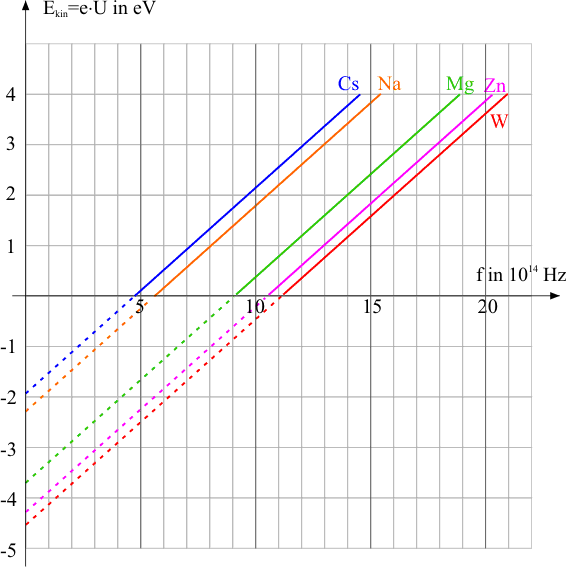
\includegraphics[width=0.5\textwidth]{img/wirkungsquantum01_quantenobjektp_ver.png}
					\caption{Graphische Auswertung der Gegenfeldmethode}
					\label{img:wirkungsquantum01_quantenobjektp_ver}
				\end{figure}
				\noindent Offensichtlich ist $\frac{\Delta E_{kin}}{\Delta f}$ konstant. Dieser Zusammenhang wird als das \textit{Planck'sche Wirkungsquantum} beschrieben. Außerdem ist es Materialabhängig, wie viel Energie benötigt wird, um Elektronen aus den Metallplatten zu lösen. Diese Energie wird als die Austrittsenergie $E_A$ bezeichnet. Wir haben also folgenden Zusammenhang:
				
				\begin{equation}
					h\cdot f=E_{kin}+ E_A
				\end{equation}
				Durch den Energieerhaltungssatzes und des Wissens, dass nirgends Energie verloren ging oder abgesehen von dem Licht dem System keine Energie zugeführt wurde muss $E_{kin}+ E_A=E_{Ph}$ gelten. Damit haben wir einen Zusammenhang zwischen der Frequenz und der Energie eines Photons:
				
				\begin{equation}
				h\cdot f=E_{Ph}
				\end{equation}
				Mithilfe des Graphen aus Abbildung \ref{img:wirkungsquantum01_quantenobjektp_ver} lässt sich das Planck'sche Wirkungsquantum als
				\begin{equation}
				h = 6.6397 \cdot 10^{-24} \si{\joule\second}
				\end{equation}
				bestimmen.
				
				
			
			\subsubsection{Röntgenspektren}
			
				\paragraph{Bragg-Bedingung}
				\begin{figure}[H]
					\centering
					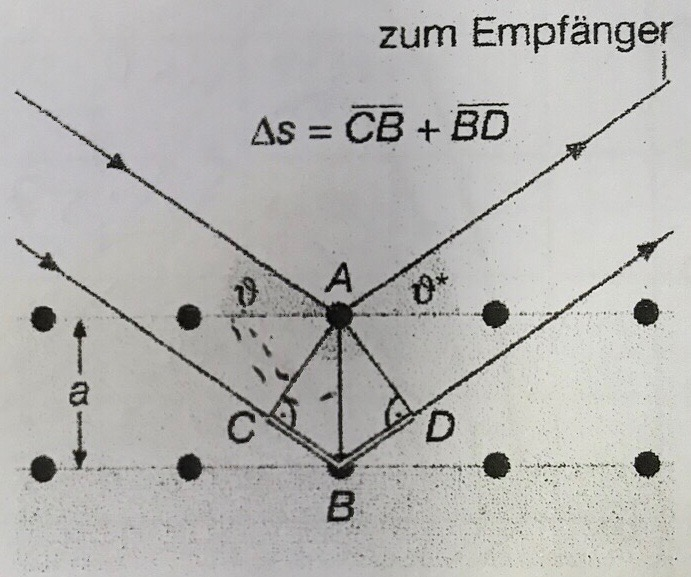
\includegraphics[width=0.5\textwidth]{img/Interferenz_am_Kristall.jpg}
					\caption{Bragg-Bedingung}
					\label{img:Interferenz_am_Kristall}
				\end{figure}
				\noindent Die Bragg-Bedingung beschreibt, welche Wellenlängen bei der Reflektion am Kristall wie in Abbildung \ref{img:Interferenz_am_Kristall} zu sehen ist verstärkt werden. Damit sich die Wellen konstruktiv überlagern, muss wie beim Doppelspalt $\Delta s = k\cdot \lambda, k\in \mathbb{N}$ erfüllt sein. Dabei ist $\Delta s = |\overline{CB}| + |\overline{BD}|$. Da $|\overline{CB}| = |\overline{BD}|$ gilt, kann folgender Zusammenhang aufgestellt werden:
				
				\begin{equation}
					\begin{aligned}
						\frac{\Delta s}{2} &= |\overline{CB}|\\
						\frac{\Delta s}{2} &= a\cdot sin(\vartheta)\\
						k\cdot \lambda &= 2a\cdot sin(\vartheta), k\in \mathbb{N}
					\end{aligned}
				\end{equation}
			
			
				\begin{figure}[H]
					\centering
					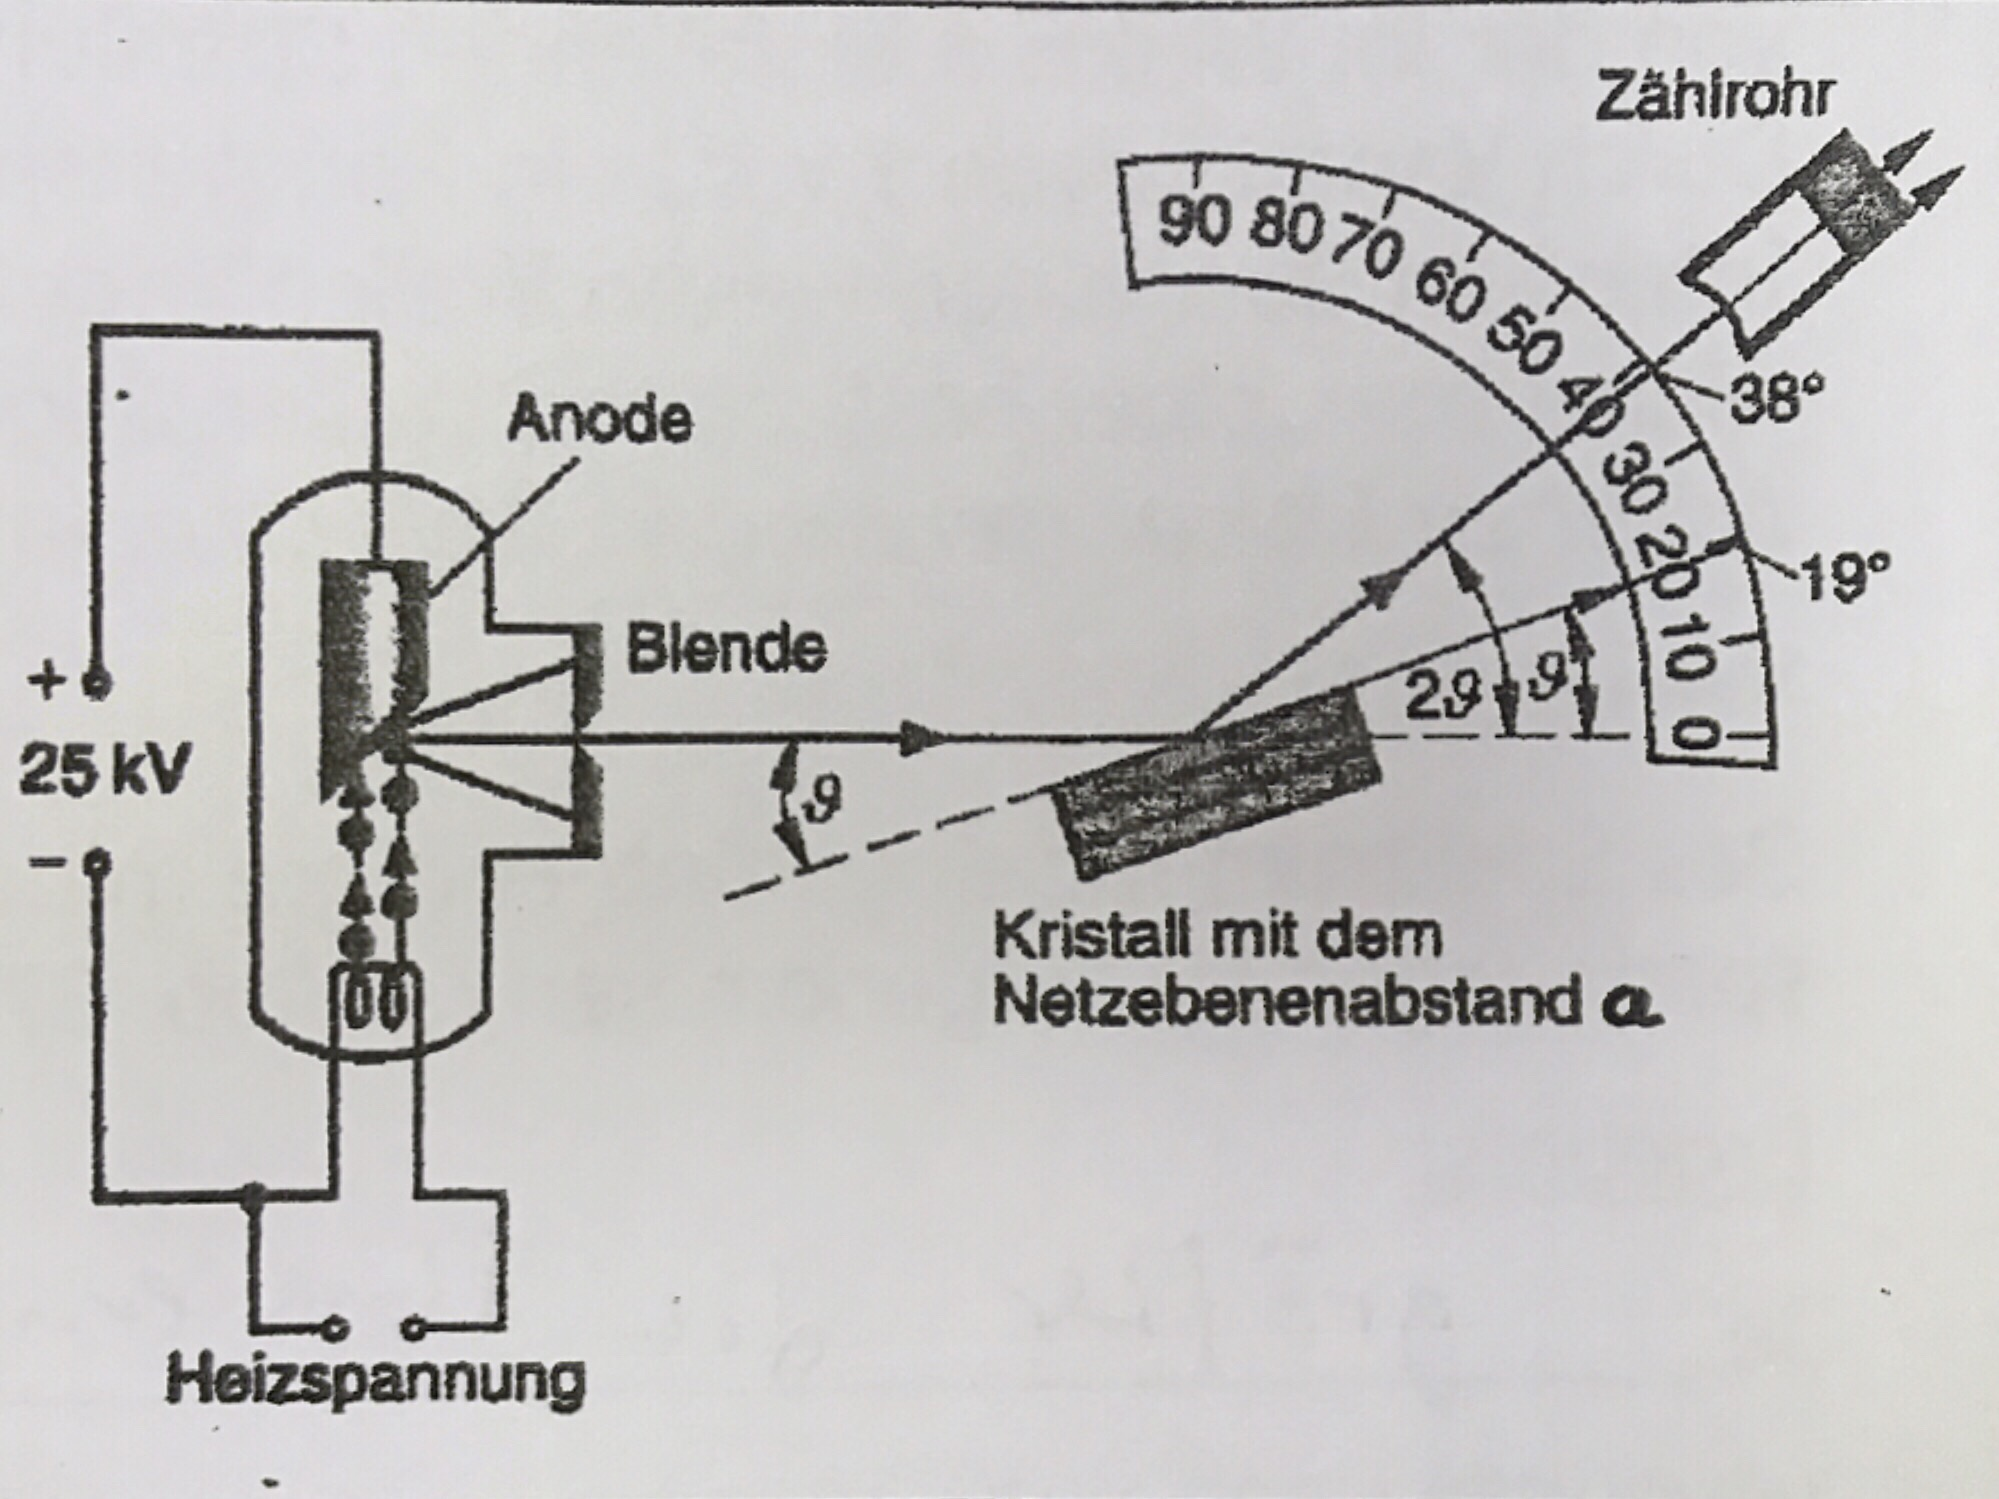
\includegraphics[width=0.5\textwidth]{img/roentgenstrahlung_aufbau.jpg}
					\caption{Aufbau der Röntgenspektrenanalyse}
					\label{img:roentgenstrahlung_aufbau}
				\end{figure}
			\noindent Die Röntgenröhre (vergleiche Abbildung \ref{img:roentgenstrahlung_aufbau}) besteht aus zwei Teilen. Auf der linken Seite werden Elektronen mit einer Heizspannung emittiert und anschließen mit hier $25\si{\kilo\volt}$ beschleunigt. Die Elektronen mit der Energie $E_{kin} = Q\cdot U = e\cdot U$ treffen auf die $45\si{\degree}$ angeschrägte Anode. Dabei entsteht die sogenannte Bremsstrahlung. Diese wird nun auf einen Kristall gerichtet, der nach der Bragg-Bedingung genau eine Wellenlänge reflektiert. Diese kann mit einem Zählrohr gemessen werden. Führt man dies für alle Winkel $0\le \vartheta \le \frac{\pi}{4}$ und verschiedene Beschleunigungsspannungen durch, erhält man die in Abbildung \ref{img:roentgenspektren_auswertung} dargestellten Graphen.
			
	
			\begin{figure}[H]
				\centering
				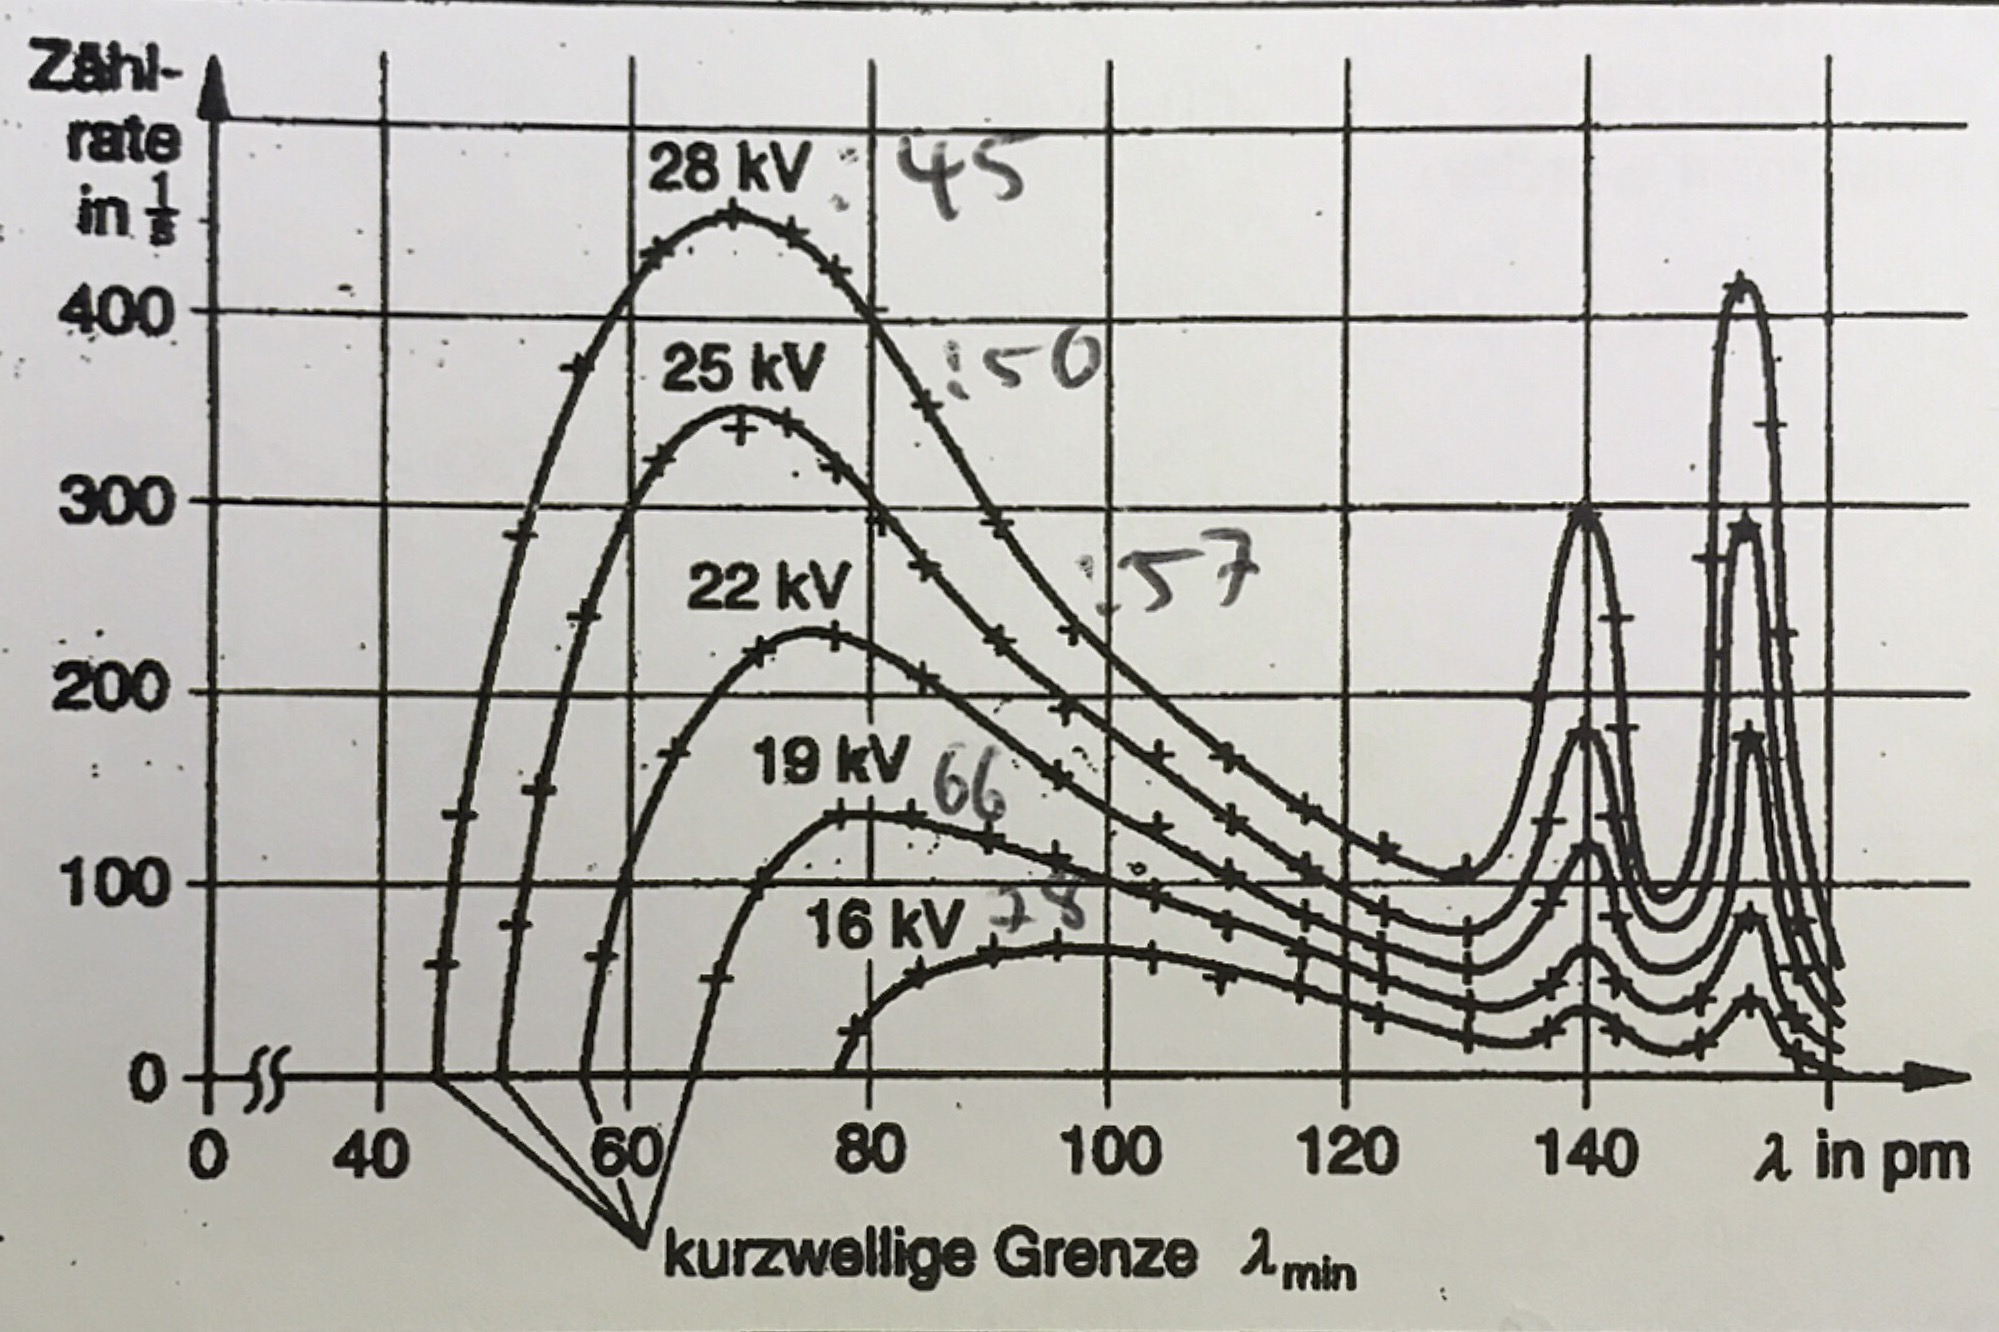
\includegraphics[width=0.5\textwidth]{img/roentgenspektren_auswertung.jpg}
				\caption{Auswertung der Röntgenröhre}
				\label{img:roentgenspektren_auswertung}
			\end{figure}
		
			\noindent Man kann erkennen, dass es eine minimale Wellenlänge $\lambda_{min}$ gibt. Offensichtlich erhält ein Photon eine maximale Energiemenge. Durch den Energieerhaltungssatz ist bekannt, dass dies maximal $E_{Ph} = E_{kin}$ sein kann. Nun kann man die minimale Wellenlänge folgendermaßen bestimmen:
			
			\begin{equation}
				\begin{aligned}
					\lambda_{min} &= \frac{c}{f_{max}}\\
					&= \frac{c}{\frac{E_{kin}}{h}}\\
					&= \frac{c\cdot h}{E_{kin}}\\
					&= \frac{c\cdot h}{e\cdot U}\\
				\end{aligned}
			\end{equation}
			
		\subsection{Lichtquantenhypothese}
		\begin{enumerate}
			\item Die Energie elektromagnetischer Strahlung mit der Frequenz $f$ wird durch quantisierte – also nicht teilbare Energieportionen (\textit{Photonen}) der Größe $E_{Ph} = h\cdot f$ übertragen.
			\item Ein Elektron absorbiert jeweils die Energie eines Photons.
			\item Helles Licht, also Licht mit hoher Intensität hat mehr Photonen, nicht aber Photonen größerer Energie.
			\item Energiereiches (kurzwelliges) Licht hat Photonen größerer Energie.
		\end{enumerate}				
			
		\subsection{Masse und Impuls von Photonen}
			Legt man die von Einstein veröffentlichte Gleichung $E=m\cdot c^2$ zugrunde kann man folgendermaßen die Masse und den Impuls eines Photons berechnen:
			
			\begin{equation}
				\begin{aligned}
					E&=m\cdot c^2\\
					m &= \frac{E}{c^2}\\
					&= \frac{h\cdot f}{c^2}
				\end{aligned}
			\end{equation}
			Die Masse kann man nachweisen, indem man die Rotverschiebung von Photonen, die sich von einer großen Masse wie einem Stern entfernen, zeigt. Dies passiert, da sie von der Gravitation beeinflusst werden und sich ihre kinetische Energie verändert.\\
			Nun kann man auch mit der Gleichung $p=m\cdot v$ aus der klassischen Mechanik den Impuls bestimmen:
			\begin{equation}
				\begin{aligned}
					p&=m\cdot v\\
					&=\frac{h\cdot f}{c^2}\cdot c\\
					&=\frac{h\cdot f}{c}\\
					&=\frac{h}{\lambda}\\
				\end{aligned}
			\end{equation}
			
								
			
		\subsection{Compton Effekt}
			Beim Compton Effekt lässt man ein Photon mit der Wellenlänge $\lambda$ und dem Impuls $\vec{p_{Ph}}$ auf ein sich in Ruhe befindendes Elektron treffen. Nah dem ''Stoß'' bewegt sich das Photon unter dem Streuwinkel $\vartheta$ mit der neuen größeren Frequenz $\lambda'$ und dem vom Betrag her geringeren Impuls $\vec{p_{Ph}'}$. Das Elektron bewegt sich dann mit dem Impuls $\vec{p_{e}'}$. Dabei muss nach dem Impulserhaltungssatz $\vec{p_{Ph}}=\vec{p_{Ph}'} + \vec{p_{e}'}$ gelten. Die Wellenlängenänderung des Photons ist bei dem Stoß
			
			\begin{equation}
				\Delta\lambda = \lambda'-\lambda = \lambda_c\cdot(1-\cos(\beta)), \lambda_c = \frac{h}{m_e\cdot c}
			\end{equation}
			
	\section{Quantenobjekte}
		\subsection{Eigenschaften von Photonen}
			\begin{enumerate}
				\item Interferenzfähigkeit mit sich selbst
				\item Interferenzmuster aus diskreten Lokalisationspunkten
				\item Bestimmt (also mess- und berechenbar) ist die Verteilung der Lokalisationspunkte nach Wahrscheinlichkeitsgesetzen. Die Ermittlung erfolgt durch Zeigeraddition bei Umdeutung der
				\subitem resultierenden Amplitude $\hat{y}$ zur Wahrscheinlichkeitsamplitude $|\Psi|$ und der
				\subitem Intensität $\hat{y}^2$ zur Antreffwahrscheinlichkeit $|\Psi|^2$.
				\item Der Weg von der Quelle zum Lokalisationspunkt ist unbestimmt. Alle möglichen Wege sind gleichberechtigt (Superposition).
			\end{enumerate}
		\subsection{Komplementarität}
			Es ist nicht möglich sowohl den Weg eines Quants zu verfolgen als auch ein Interferenzbild zu erhalten. Man kann also nicht das Teilchen und Wellenmodell gleichzeitig anwenden, man braucht aber beide, da man nicht alle Effekte mit einem der beiden erklären kann.
		\subsection{Superposition}
			Da die Bahn eines unteilbaren Quants zu einem Ort unbestimmt ist, müssen alle möglichen Bahnen als Rechenpfade mit $\lambda$-Zählern berücksichtigt werden. Das Superpositionsprinzip verbindet das Teilchen und das Wellenmodell miteinander.
		\subsection{Knallertest}%TODo einbauen: Knallertest
		\subsection{Teilchen als Quantenobjekte}%TODo vervollständigen
		De-Broglie stellte die Hypothese auf, dass sich Teilchen wie Elektronen ebenfalls wie Quantenobjekte ausbreiten. Die Experimente von Jonsson zeigten dies, da Elektronen ein Interferenzmuster an einem Doppelspalt erzeugten.
		

\end{document}